% Co jsem udělal já
\chapter{Návrh zařízení}
\section{Princip funkce navrženého systému}\label{sec:PopisFunkceSystemu}
% \purpose{Tady bych rád popsal, jak to bude celé fungovat.}

Celý systém je primárně navržen kolem mobilní aplikace, jelikož požadavek na dálkové řízení dopravníků je jeden ze základních požadavků navrženého systému.

Aplikace bude obsahovat stránku pro plynulou WiFi komunikaci s vývojovou deskou WEMOS D1 Mini Pro. Vývojová deska je připevněna k desce plošných spojů, která je třemi kabely připojena na ovládací panel (2 datové kabely a 1 napájecí). Tímto způsobem může deska nastavovat takové digitální vstupy, k ovládání dopravníku.

Ovládací panel frekvenčního měniče si následně dle jeho nastavení podle své konfigurace interpretuje tyto příkazy a řídí výkonovou část frekvenčního měniče pro ovládání asynchronních motorů.

Na obrázku \ref{fig:PrincipFunkceZarizeni} je schéma základního principu.

\begin{figure}[hptb]
	\centering
	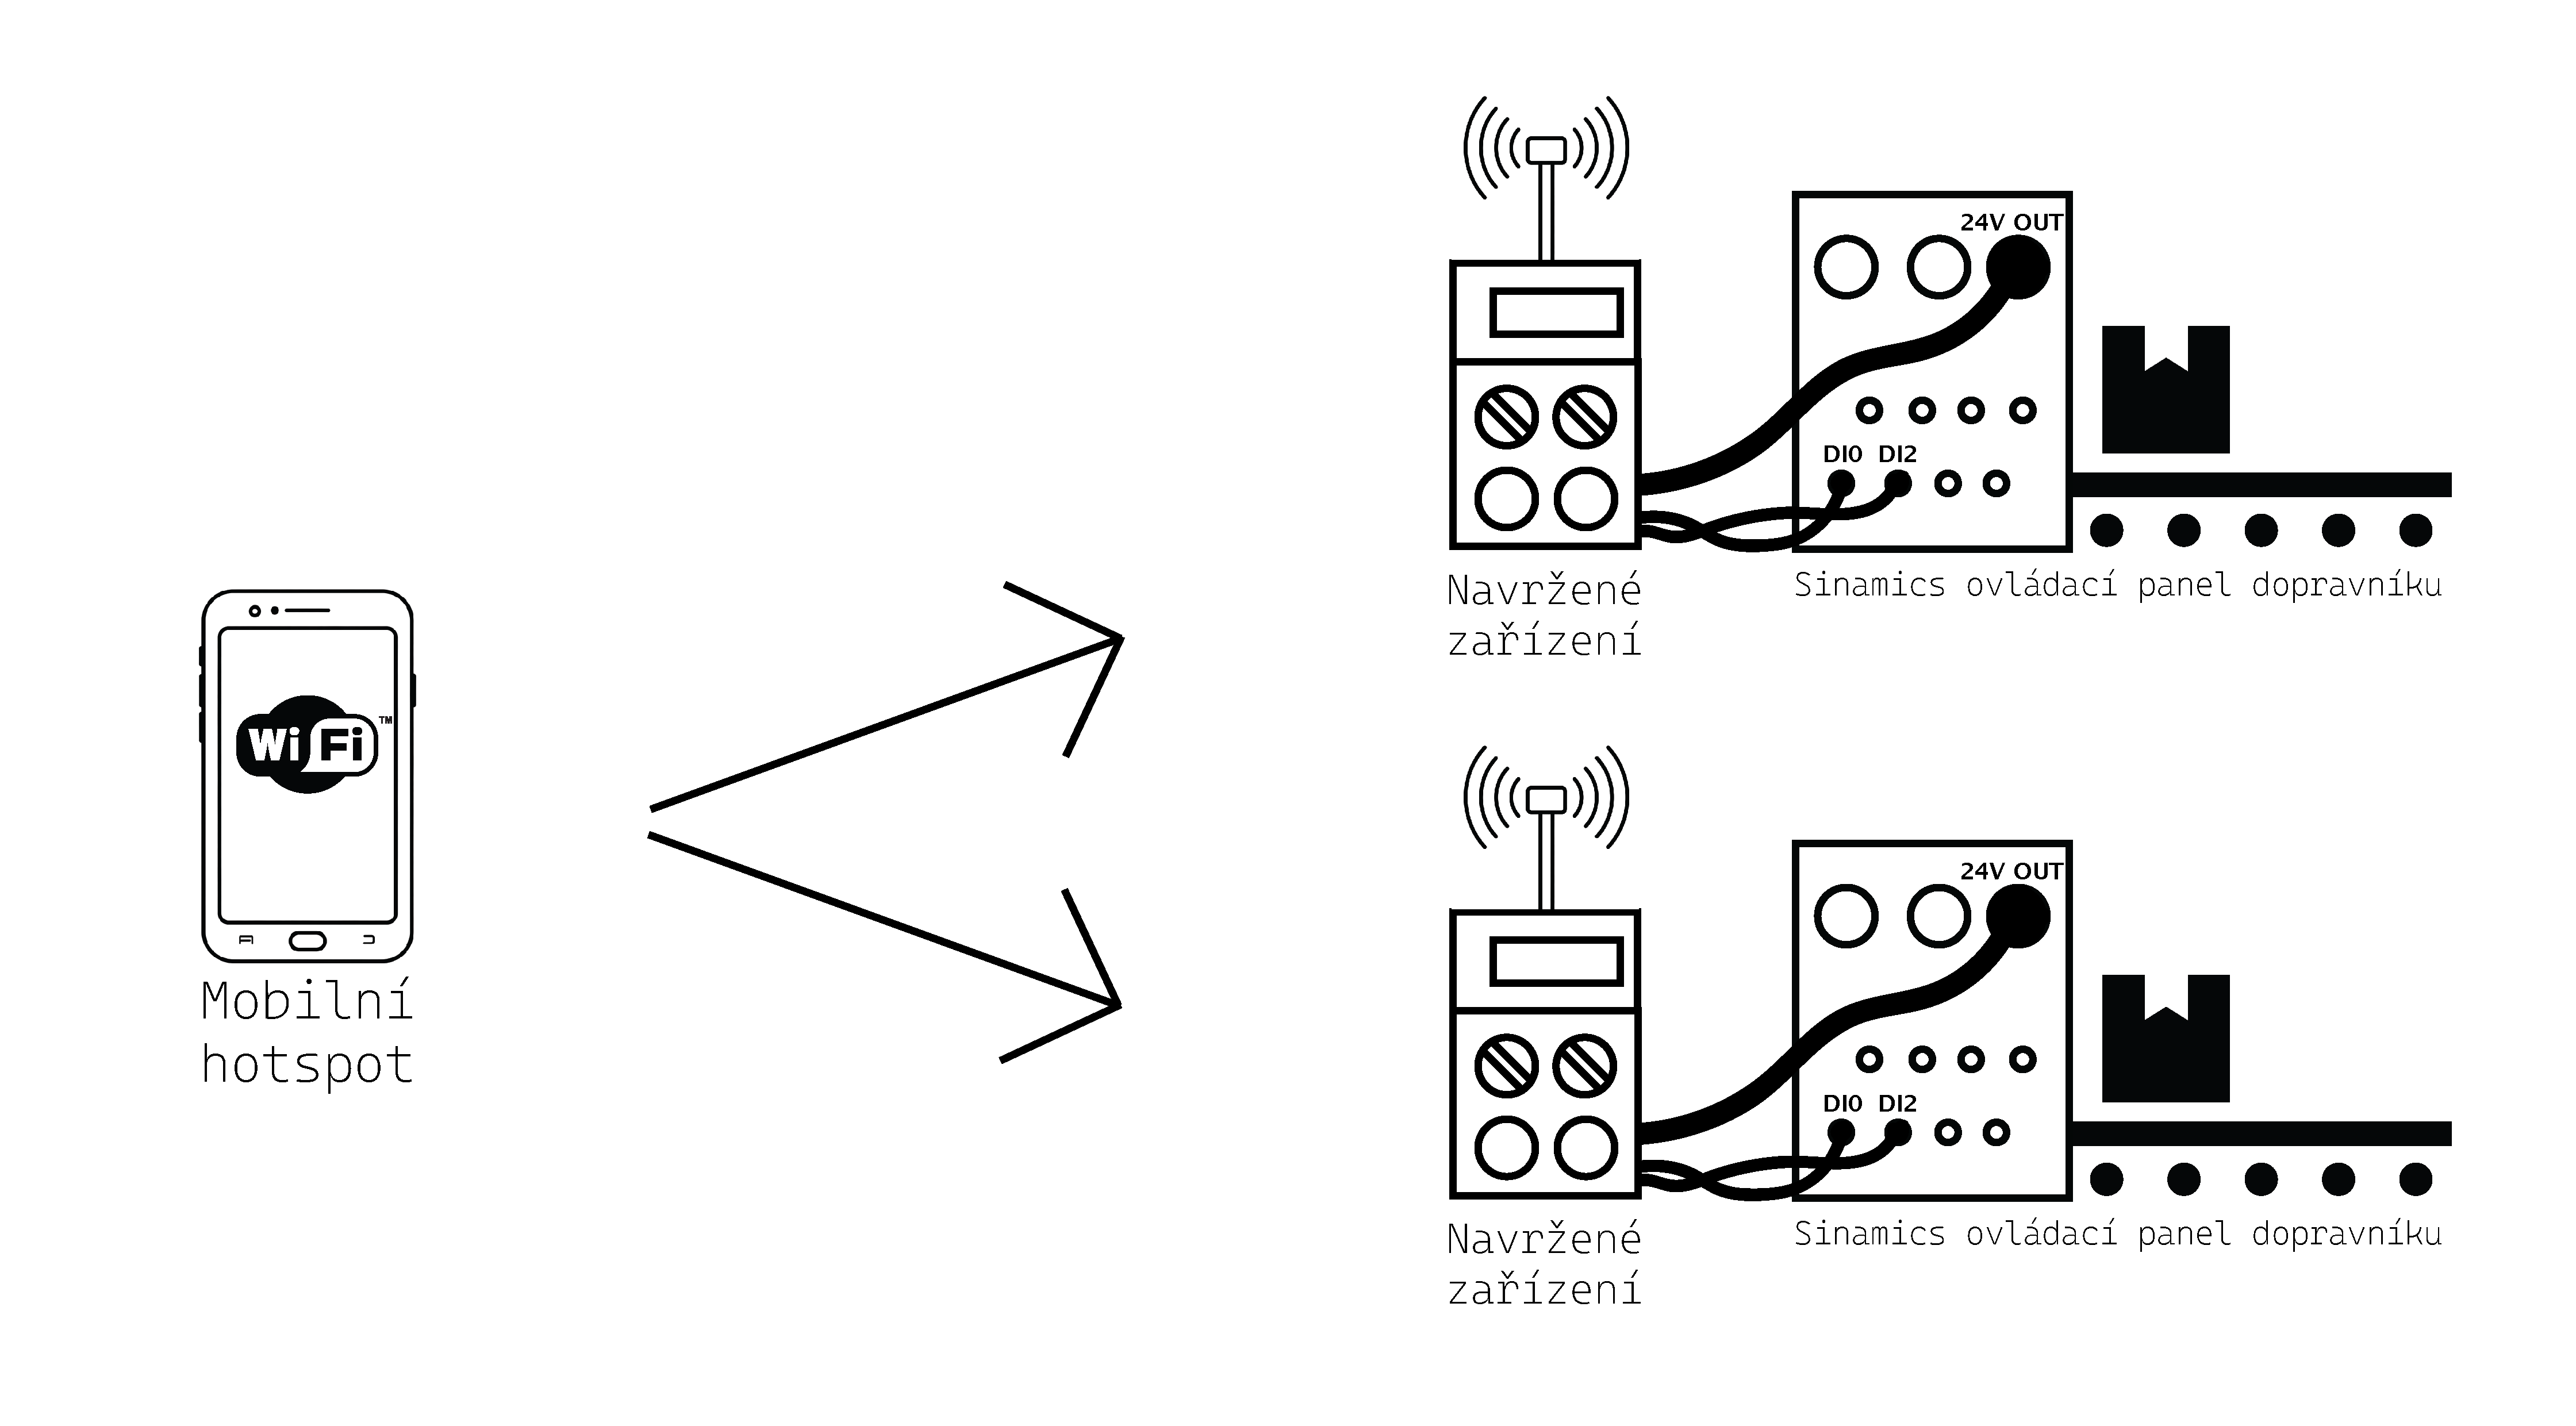
\includegraphics[width=1\linewidth]{images/FunkcniSchema_DvaOvladace.png}
	\caption{Schéma principu jak navržený systém funguje}
	\label{fig:PrincipFunkceZarizeni}
\end{figure}

Jelikož mobilní aplikace komunikuje s vývojovými deskami pomocí WiFi, je potřebné aby se buďto mobilní zařízení připojilo na přístupové místo vývojové desky, anebo se může vývojová deska připojit na hotspot mobilního zařízení. WebServer umožňuje obě varianty. Pro účely tohoto systému se více hodí ta druhá možnost, protože přirozeně umožňuje mít jeden hotspot na mobilním zařízení a na ten se může připojit více vývojových desek. Tohle umožňuje jednoduše ovládat více dopravníků zároveň. Další výhoda je, že vývojové desky připojené na hotspot vůbec nevyužívají toho, že je mobilní telefon připojený k internetu a tak nijak nezatěžují rychlost připojení - jediná limitace počtu takto připojených vývojových desek je tedy limitace maximálního počtu co může mít mobilní telefon připojené přes hotspot. Nevýhoda tohoto způsobu komunikace je ovšem taková, že se musí nastavit jednotné jméno a heslo WiFi komunikace, které bude zadané přímo ve firmwaru vývojové desky a pokud bude potřebné tyhle údaje změnit, bude se muset přehrát kód všech vývojových desek (pro všech pět používaných zařízení).

Díky tomu, že je tento systém navržený tak, aby přes 5-pinové kabely spínal digitální vstupy ovládacího panelu, je tento systém možné použít i na frekvenční měniče jiných značek než je Sinamics. Kabely, které se používají pro komunikaci s ovládacím panelem frekvenčního měniče (M12 5-pinové kabely) jsou v dnešní době u frekvenčních měničů časté. Jediné co je tedy potřeba pro používání systému s jiným frekvenčním měničem jsou správné konektory a dále aby bylo možné vyresetovat ovládací panel do podobného výchozího nastavení jako má Sinamics CU240-2.

Na obrázku \ref{fig:PopisZarizeniCoOvladaDopravnik}  je finální vzhled schránky na desku plošných spojů s tlačítky, LCD displejem a dalšími funkcemi. Deska je dále popsaná v kapitole \ref{sec:Hardware}.

\begin{figure}[hptb]
	\centering
	\includegraphics[width=0.7\linewidth]{images/obrazekKrabicky_annot.png}
	\caption{Popis zařízení co ovládá dopravník}
	\label{fig:PopisZarizeniCoOvladaDopravnik}
\end{figure}

Na obrázku \ref{fig:MobilniAppScreenshots} je finální vzhled mobilní aplikace. Jsou zde vidět tři hlavní strany aplikace - Nastavení, Pomoc a Ovládání. Ovládání komunikuje s vývojovou deskou tím že posílá příkazy pro ovládání dopravníku, ale také získává průběrná data o rychlosti dopravníku a typu ovládání (lokální nebo dálkové). Aplikace je dále popsaná v kapitole \ref{sec:SoftwareVMobilniAplikaci}.

\begin{figure}[hptb]
	\centering
	\begin{subfigure}[t]{0.3\textwidth}
		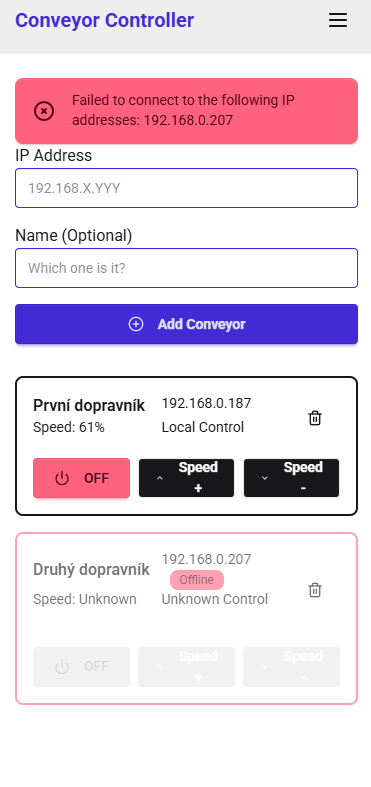
\includegraphics[width=\textwidth, height=290px]{images/MobilniLanding.png}
		\caption{Vstupní stránka aplikace}
		\label{fig:MobilniLanding}
	\end{subfigure}%
	\begin{subfigure}[t]{0.3\textwidth}
		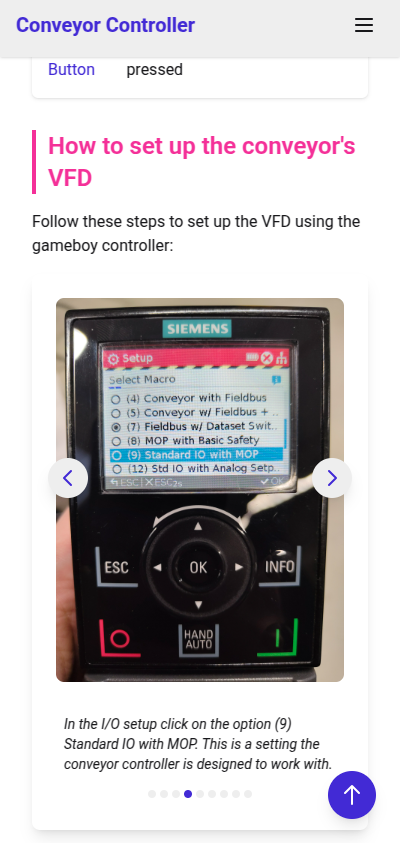
\includegraphics[width=\textwidth, height=290px]{images/MobilniSetup.png}
		\caption{Část stránky nastavení}
		\label{fig:MobilniSetup}
	\end{subfigure}%
	\begin{subfigure}[t]{0.3\textwidth}
		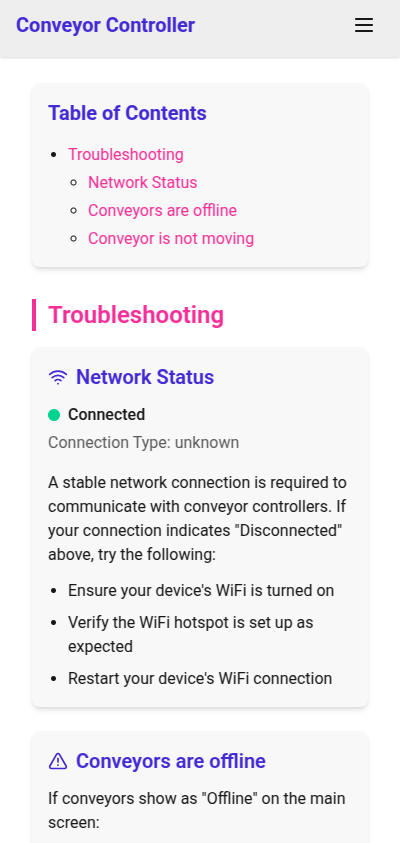
\includegraphics[width=\textwidth, height=290px]{images/MobilniHelp.png}
		\caption{Část stránky s častými chybami}
		\label{fig:MobilniHelp}
	\end{subfigure}
	\caption{Vysílat příkazy zařízení bude mobilní aplikace připojená přes hotspot}
	\label{fig:MobilniAppScreenshots}
\end{figure}

\subsection{Požadavky na systém}\label{sec:PozadavkyNaSystem}
Pro zajištění funkčnosti a smysluplnosti návrhu je nutné si stanovit některé požadavky, které by systém měl splňovat. Tyto požadavky reflektují nejenom požadavky od společnosti Honeywell, ale i požadavky na základní spolehlivost, jednoduchost a bezpečnost ovládání dopravníků tímto způsobem.

Zde jsou požadavky, které by implementace navrženého zařízení měla splňovat:

\begin{itemize}
    \item \textbf{Lokální a dálkové ovládání}\\
    Systém bude schopný ovládat dopravníky nejenom lokálně ale i bezdrátově.
    \item \textbf{Ovládání více dopravníků zároveň}\\
    Systém by měl jednoduše zprostředkovat ovládání více dopravníků zároveň.
    \item \textbf{Ovládání z mobilního zařízení}\\
    Aby se minimalizoval počet potřebných zařízení se systém musí dát provozovat z mobilního zařízení pomocí WiFi hotspotu.
    \item \textbf{Napájení z ovládacího panelu}\\
    Systém musí být navržený tak aby jeho rozšířené funkce bylo možné napájet připojením na $24V$ výstupní port v ovládacím panelu.
    \item \textbf{Systém musí mít ovládání které je čistě analogové}\\
    Systém by měl být navržen tak, aby bylo stále možné dopravníky ovládat i pokud by něco zamezovalo napájení vývojové desky.
    \item \textbf{Uživatelská přívětivost systému}\\
    Systém by měl být uživatelsky přívětivý a jeho nastavení by mělo být jednoduše dostupné pro uživatele spolu se všemi informacemi jak s ním pracovat.
\end{itemize}

\section{Hardware}\label{sec:Hardware}
% \purpose{Jak jsem postupoval při návrhu a jak ta finální verze vypadá}

Základní stavební kámen celého systému je jeho hardware společně s deskou plošných spojů (DPS) ve které je umístěn. Celé zapojení bylo nejdříve navržené jako elektrické schéma. To bylo postupně vylepšováno, později předěláno do schématu v programu pro tvorbu DPS a nakonec bylo vytvořené rozložení komponentů přímo na desce. Pozdější verze návrhu byly provedeny v počítačovém programu na návrh desek plošných spojů jménem KiCAD. Blokové schéma funkčnosti desky lze vidět na obrázku \ref{fig:SchemaDesky}.

\begin{figure}[hptb]
	\centering
	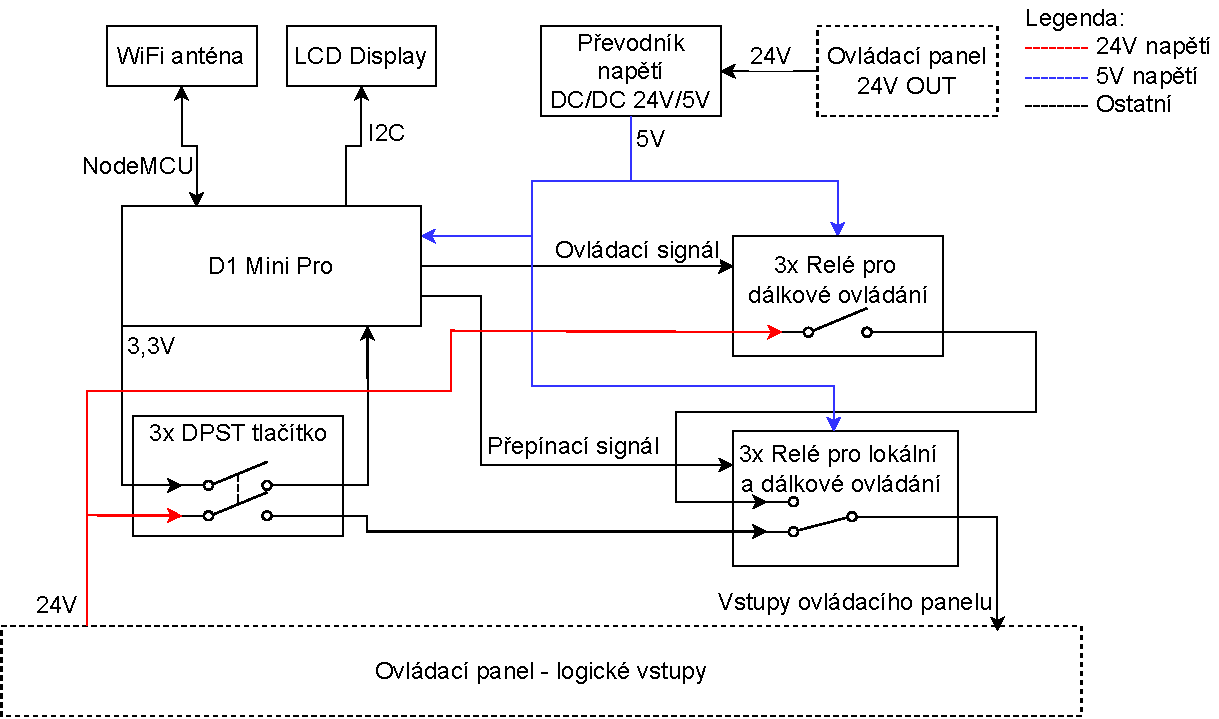
\includegraphics[width=1\linewidth]{images/Electrical_Schematic_V2.drawio.pdf}
	\caption{Blokové schéma desky plošných spojů}
	\label{fig:SchemaDesky}
\end{figure}

Při tvorbě desky se vycházelo z požadavků na systém. Nejdřív se vycházelo z toho, že desku musí být možné napájet z ovládacího panelu, který má výstupní port na kterém je $24V$ a který je schopný dodat maximálně $8A$. Ze začátku se tedy počítalo s $24V$ napětím, pro které bylo potřeba zvolit dobrý převodník napětí co je schopný napětí přeměnit na $5V$ kterým se napájí vývojová deska. Nakonec byl zvolený převodník napětí s galvanicky oddělenou zemí aby se minimalizovala šance, že by kvůli nějaké chybě v návrhu desky byl zničený ovládací panel frekvenčního měniče.
\cite{SiemensG120DGettingStarted}

Dále se při návrhu vycházelo z myšlenky že systém musí mít i lokální i dálkové ovládání, s tím, že lokální ovládání musí být dostupné i bez napájení mikrokontroleru. Tohle bylo vyřešeno návrhem dvou přepínačů. \textit{Relé pro lokální a dálkové ovládání} je přepínač, který je normálně v poloze lokálního ovládání (aby byl splněný požadavek čistě analogového ovládání), ale pokud se na něj přidá napětí a dostatečný proud, přepne se do stavu dálkového ovládání. Následně je v desce \textit{Relé pro dálkové ovládání}, což je běžné SPST relé, které sepne kontakty pokud je na něj přivedeno napětí a dostatečný proud.

Po dokončení schématu se přešlo na návrh umístění součástek na DPS. Finální návrh lze vidět v obrázku \ref{fig:PCBbothSides}. Při rozmisťování součástek po desce byl kladen důraz na několik kritérií:
\begin{itemize}
	\item Aby měla deska co nejmenší rozměry a jen dvě vrstvy.
	\item Aby byly všechny součástky na jedné straně desky (jednodušší pájení komponentů na desku).
	\item Aby byly trasy co nejkratší.
	\item Aby měla deska co nejméně vertikálních cest (pro zmenšení efektů parazitní kapacity a parazitní indukčnosti).
	\item Aby byly filtrační kondenzátory co nejblíž filtrovaných napájecích vstupů.
\end{itemize}

\begin{figure}[hptb]
	\centering
	\begin{subfigure}[t]{0.48\textwidth}
		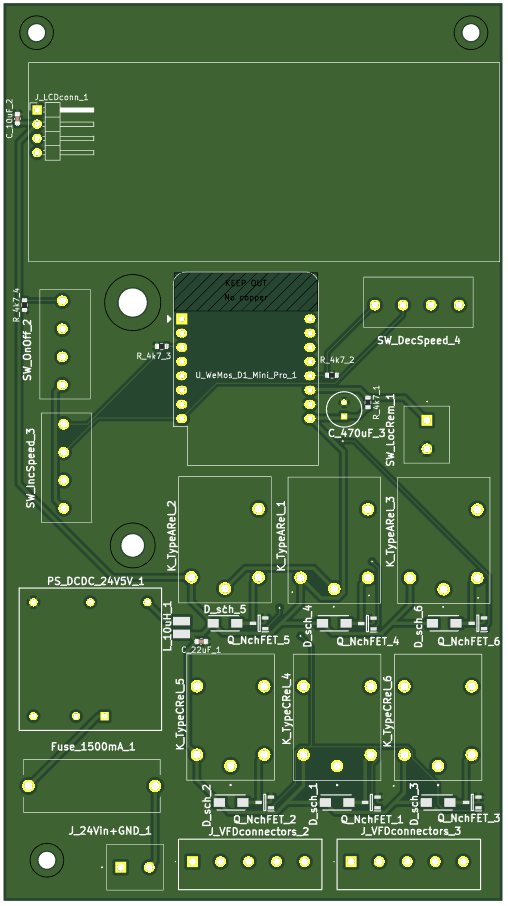
\includegraphics[width=\textwidth]{images/PCBfront.png}
		\caption{Přední strana DPS}
		\label{fig:PCBfront}
	\end{subfigure}%
	\hfill
	\begin{subfigure}[t]{0.48\textwidth}
		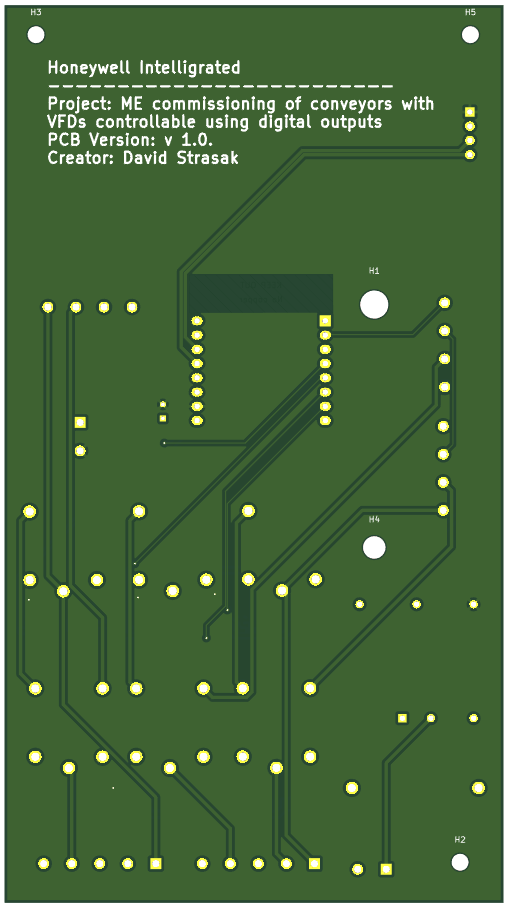
\includegraphics[width=\textwidth]{images/PCBback.png}
		\caption{Zadní strana DPS}
		\label{fig:PCBback}
	\end{subfigure}
	\caption{Návrh desky plošných spojů v KiCAD}
	\label{fig:PCBbothSides}
\end{figure}

\subsection{Ovládání relé}
Jedna z věcí které bylo potřeba vyřešit při návrhu schématu elektrického obvodu je taková, že bylo cílem ovládat relé pomocí výstupních pinů vývojové desky. Pro spuštění relé je ovšem potřeba brát na paměť, že vyžaduje nejenom napětí $5V$ na ovládacím pinu, ale také vyžaduje proud do cívky $133mA$. Vývojová deska je schopná svými výstupními piny poskytnout napětí $5V$, ale její výstupní proud je pouze $10mA$. Tento problém je možné vyřešit pomocí tranzistorů.

Nejjednodušší řešení pro navrženou desku je řešení s N kanálovým NPN tranzistorem MOSFET, jelikož v případě MOSFET tranzistorů obecně stačí aby signál byl napěťový (nemusíme tedy řešit malý proud vycházející z vývojové desky). Nejdřív se relé zapojí tak, aby cívka měla na jedné straně $5V$ napětí a na druhé straně zem. Následně se MOSFET tranzistor dá mezi zem a cívku a na bázi tranzistoru se přivede signál z mikrokontroleru. V tomto zapojení bude skrz relé téct nominální proud, pokud je výstup vývojové desky vysoký, anebo bude obvod rozpojený pokud bude výstup z vývojové desky na nízké hodnotě napětí.

Dále je potřeba ještě paralelně s relé zapojit diodu kvůli ochraně tranzistoru od vybíjecího proudu co cívka generuje po rozpojení obvodu. Tato dioda musí mít v závěrném směru hodnotu napětí vyšší než je $5V$ napětí zdroje a musí se zapojit tak, aby byla otevřená když se otočí polarita napětí na cívce v relé. Pro tuto desku byla zvolena Schottkyho dioda kvůli její rychlosti přepínání a kvůli malému napětí které se na diodě v otevřeném stavu nachází.

Na obrázku \ref{fig:OvladaniRele} je schéma zapojení tohoto způsobu ovládání relé pomocí vývojové desky.

\begin{figure}[hptb]
	\centering
	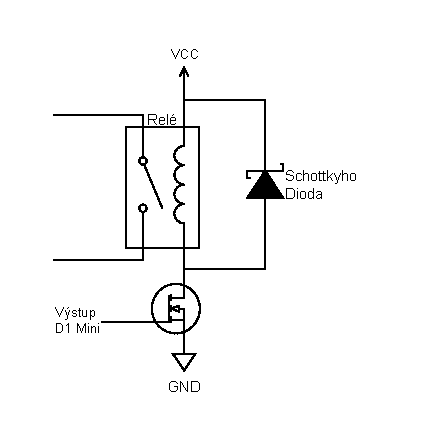
\includegraphics[width=0.6\linewidth]{images/OvladaniRele.drawio.pdf}
	\caption{Elektrické schéma ovládání relé}
	\label{fig:OvladaniRele}
\end{figure}

\subsection{LCD display s I2C převodníkem}
Aby bylo možné celý systém ovládat přes ESP8266 WebServer, je potřebné nějakým způsobem komunikovat s uživatelem IP adresu, kterou má vývojová deska připojená na hotspot mobilního zařízení. Tohle by bylo možné udělat například skrz nastavení multicast DNS na specifickou adresu a tu potom fyzicky napsat na schránku desky. Toto řešení by sice umožnilo přístup k WebServeru, ale neposkytovalo by to další funkce jako systém může mít se zabudovaným LCD displejem do desky plošných spojů.

Použití LCD displeje v systému může uživateli dodávat tyto informace:
\begin{itemize}
	\item Stav připojení mikrokontroleru k hotspotu (před navázáním spojení systém nemůže reagovat na požadavky přes WebServer).
	\item Název (SSID) a heslo hotspotu, které mikrokontroler očekává.
	\item Aktuální rychlost dopravníku.
	\item IP adresu pro přístup k WebServeru.
\end{itemize}

Na základě uvedených důvodů a požadavků na rozsah poskytovaných informací byl pro komunikaci s uživatelem zvolen LCD displej.

Konkrétně byl použit 16x2 znakový LCD displej (obrázek \ref{fig:LcdDisplej}) zakoupený v internetovém obchodě LaskaKit \cite{laskakit_16x2_lcd}. Tento model je vybaven připájeným I2C převodníkem, což zjednodušuje jeho připojení na pouhé čtyři vodiče: dva pro I2C sběrnici (Serial Data (SDA) a Serial Clock (SCL)), jeden pro napájení $5V$ a jeden zemnící vodič (GND). Výhodou zvoleného displeje je také dostupnost knihovny pro Arduino framework, což usnadňuje jeho softwarovou implementaci ve firmwaru mikrokontroleru.
\cite{laskakit_16x2_lcd}

\begin{figure}[hptb]
	\centering
	\begin{subfigure}{0.48\textwidth}
		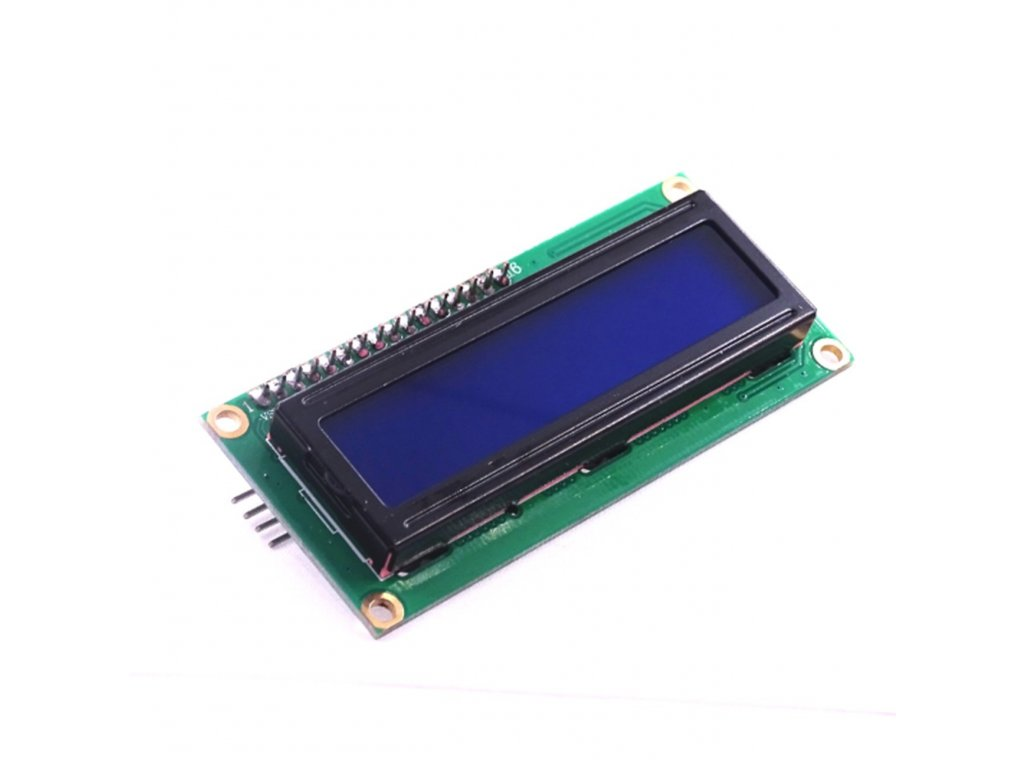
\includegraphics[width=1\textwidth]{images/predni_LCD_s_I2C.jpg}
		\caption{Přední strana}
		\label{fig:PredniLCDDisplej}
	\end{subfigure}
	\hfill
	\begin{subfigure}{0.48\textwidth}
		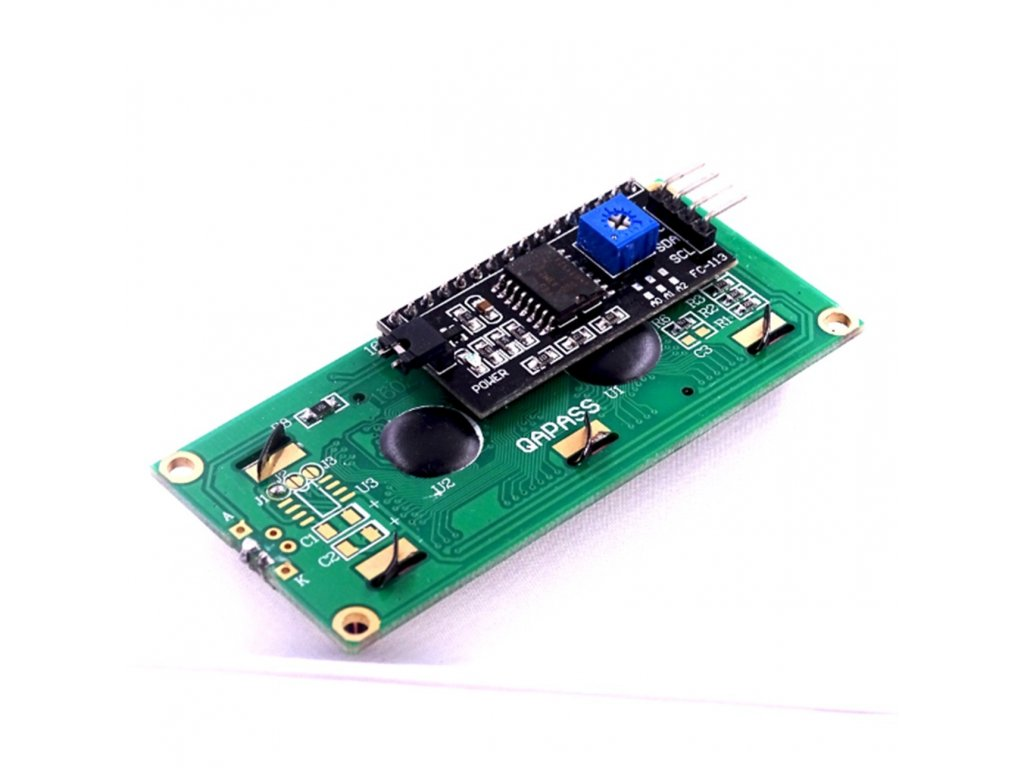
\includegraphics[width=1\textwidth]{images/zadni_LCD_s_I2C.jpg}
		\caption{Zadní strana}
		\label{fig:ZadniLCDDisplej}
	\end{subfigure}
	\caption{LCD displej s I2C převodníkem \cite{laskakit_16x2_lcd}}
	\label{fig:LcdDisplej}
\end{figure}

Vzhledem k citlivosti komunikace po I2C sběrnici na elektromagnetické rušení a přeslechy byly při návrhu desky plošných spojů dodrženy zásady pro minimalizaci smyčkové plochy mezi signálovými cestami SDA a SCL. Tento postup snižuje indukované napětí a přispívá ke spolehlivosti přenosu dat na sběrnici.
\cite{CurrentLoopsBlog}

Pro jednoduchost výměny LCD displeje bylo také zvoleno, že nebude přímo připájený v desce, ale podobně jako vývojová deska bude připojený skrz kolíkové lišty. Tohle zjednodušuje výměnu nebo upravení parametrů LCD displeje jako je jas zobrazených písmen.

% Tyhle veci nebudu popisovat, protože stačilo napsat, že mám ten převodník napětí co mění z 24V na 5V a je galvanicky oddělený. Není potřeba víc to rozepisovat
%\subsection{Převodník napětí 24V-5V (1 strana)}
%\purpose{Tady vysvětlím že používám tenhle převodník napětí, nějaký jeho specifikace, podle kterých jsem si ho zvolil. }
%\purpose{Vysvětlit jaký specifický hardware součásti jsem do desky dal a proč jsem se rozhodl je tam dát.}
%
%\subsection{LC Filtr napájecího napětí (1 strana)}
%\purpose{Sem napsat jak jsem navrhoval LC filtr za napájecím napětí, proč jsem se rozhodl použít LC filtr a třeba by se sem mohl hodit nějakej grafík přenosové funkce kdybych se nudil. Zvolil jsem si cutoff aby byl alespoň 1/10 hodnoty na které měnič dělá šum a díky tomu by měla hodnota tohoto šumu být o 20dB menší.}
%\purpose{Vysvětlit jaký specifický hardware součásti jsem do desky dal a proč jsem se rozhodl je tam dát.}

\section{Firmware ve vývojové desce}\label{sec:Firmware}
% \purpose{Tady bych rád trochu vysvětlil jak funguje software ve vývojové desce.}

Jak bylo již napsáno v kapitole \ref{sec:ArduinoFrameworkForESP8266} tento projekt byl programovaný v prostředí PlatformIO. Tohle programovací prostředí má tu výhodu v tom, že pro programování vývojových desek si stačí vybrat typ vývojové desky, kterou programuji a dané prostředí se nakonfiguruje tak, aby to bylo možné (V případě WEMOS D1 Mini Pro byl implementován Arduino framework pro ESP8266). Z tohoto prostředí tedy lze programovat jakékoliv vývojové desky a programovat je jakýmkoliv jazykem mezi které patří například Arduino jazyk anebo MicroPython. Pro firmware v tomto projektu byl zvolený Arduino framework a tak je programovací jazyk Arduino verze C++.
\cite{PlatformIOWeb}

Honeywell je anglicky mluvící firma a tak je celý firmware i software v mobilní aplikaci programovaný anglicky.

V C++ programovacím jazyku se běžně objevují dva hlavní typy souborů. Jsou to hlavičkové soubory (s koncovkou \texttt{.h}) a zdrojové soubory (s koncovkou \texttt{.cpp}). Zatímco hlavičkové soubory obsahují deklarace, jako jsou prototypy funkcí nebo definice globálních proměnných, zdrojové soubory obsahují implementace a kód který je následně kompilován a prováděn na mikrokontroleru. V tomto projektu jsou dva hlavičkové a dva zdrojové soubory.

Jeden hlavičkový soubor obsahuje definice alternativních názvů pro výstupních a vstupních piny GPIO vývojové desky aby bylo jednodušší se orientovat v kódu. Dále je zde soubor \textbf{main.cpp}, který kompilátor přirozeně vyhledává aby v něm nastavil začátek provádění kódu. Nakonec je zde zdrojový a hlavičkový soubor s názvem \texttt{ConveyorController} který definuje třídu a zdrojový kód objektu který celý systém řídí.

\subsection{Třída a objekt ConveyorController}\label{sec:ConveyorController}
% \purpose{V kódu všechno ovládám pomocí tohoto objektu, který obsahuje hodně public a private funkcí. Tady bych chtěl vysvětlit z jakýho důvodu jsem se rozhodl vývojovou desku ovládat tímto způsobem a dále vysvětlit co jednotlivé důležité metody a proměnné dělají.}

C++ je objektově orientovaný program a tak má rozsáhlé funkce pro definici vlastních tříd. Kvůli tomu je důležité rozlišovat mezi pojmy třída a objekt. Třída v C++ slouží jako abstraktní definice pro vytvoření nového uživatelsky definovaného datového typu. Objekt je na druhou stranu konkrétní instance třídy a tak má alokované místo v RAM paměti a je sledovaný jeho unikátní stav během provádění kódu.
\cite{CppObjectAndClassArticle}

Hlavní výhodou proč byl v práci použitý objektově orientovaný přístup je kvůli zavedení takzvané \textbf{enkapsulace} uvnitř kódu. Jinými slovy, umožňuje to separaci řídící logiky dopravníku od zbytku aplikačního kódu. Během implementace firmwaru vyvstala potřeba, aby určité proměnné, jako například proměnná \texttt{conveyorSpeed} reprezentující aproximaci rychlosti dopravníku či proměnná \texttt{remoteLocalState} indikující stav řízení (vzdálené/lokální), byly přístupné napříč několika funkcemi. Běžně by bylo možné tyto proměnné řešit pomocí globálních proměnných, ale to je v komplexnějších firmwarech považováno za rizikové.
\cite{EnkapsulaceVCppArikl}

V takovém případě se pro bezpečnější provádění kódu může přejít k využívání objektů. Samotný objekt je sice definovaný globálně, ale uvnitř má tři definice přístupu: \textbf{veřejný, privátní a chráněný}. Tímto způsobem se může pro jakékoliv proměnné uvnitř objektu určit, v jakých částech kódu budou dostupné, s tím, že pokud je proměnná definovaná jako veřejná, dá se získat i mimo daný objekt a na druhou stranu pokud je proměnná privátní, je možné ji získat pouze uvnitř metod objektu. Metoda je taková funkce, kterou je možné uvnitř objektu se stejnými přístupy definovat a je to kus kódu co bude provedený pokud bude metoda zavolaná. Metody které jsou veřejné je tedy možné spouštět ze skriptu \texttt{main.cpp} ve kterém existuje globální instance objektu, ale privátní metody už není možné z hlavního skriptu spouštět.

Kvůli této funkcionalitě bylo od začátku rozhodnuto, že bude kód programovaný tímto způsobem. Většina kódu bude obsažena v \texttt{conveyorController} objektu a v hlavním zdrojovém kódu budou pouze volány veřejné metody této globální instance třídy \texttt{ConveyorController}.

Aby bylo možné představit jaké funkce jsou v \texttt{ConveyorController} třídě obsaženy, zde je její definice v hlavičkovém souboru \texttt{ConveyorController.h}:

\begin{lstlisting}[language=C++, caption={Header soubor ConveyorController Objektu}, label={lst:ConveyorControllerHeader}]
#ifndef CONVEYORCONTROLLER_H
#define CONVEYORCONTROLLER_H

#include <Arduino.h>
#include <ESP8266WebServer.h>
#include <ESP8266WiFi.h>
#include <ESP8266mDNS.h>
#include <LiquidCrystal_I2C.h>
#include <WiFiClient.h>
#include "pinDefinitions.h"
#include <Ticker.h>

class ConveyorController {
public:
  ConveyorController(const char* wifiNetworkName,
    const char* wifiNetworkPassword);

  void initIO();
  void initLCD();
  void initWeb();
  void assignRoutes();
  void startWebServer();
  void startTicker();
  void handleClient();
  void updateLCD();
  void updateState();

private:
  // WiFi credentials
  const char* wifiNetworkName;
  const char* wifiNetworkPassword;

  // Web server
  ESP8266WebServer webServer = ESP8266WebServer(80);

  // LCD
  LiquidCrystal_I2C lcd = LiquidCrystal_I2C(0x27, 16, 2);

  // Ticker
  Ticker inputCheckingTicker;
  Ticker LCDUpdatingTicker;

  // Speed of the conveyor
  int conveyorSpeed = 0;

  // TRUE or FALSE state if the conveyor is controlled locally or remotely
  // remoteLocalState ? "local" : "remote"
  bool remoteLocalState = false;

  // TRUE or FALSE state if the conveyor is speeding up or no
  bool locIncSpeedState = false;
  bool remIncSpeedState = false;

  // TRUE or FALSE state if the conveyor is slowing down or no
  bool locDecSpeedState = false;
  bool remDecSpeedState = false;

  // TRUE or FALSE state if the conveyor is ON or OFF
  bool locOnOffState = false;
  bool remOnOffState = false;

  // Route handler for the main page
  void mainRoute();

  // Route handler for unknown pages
  void unknownRouteResponse();

  void LCDWaitingForConnection(bool condition);

  void writeValue(int pin, int value);
};

#endif
\end{lstlisting}


Z této definice lze vidět, že pro přehlednost je celkový kód rozdělený do různých metod tak, aby měla každá metoda svůj účel. Tyto metody jsou seřazené podle pořadí provedení až do funkce \texttt{startTicker}, po které se už funkce provádějí periodicky. Účely které zajišťují metody jsou:

\begin{itemize}
	\item \textbf{initIO} - Nastavuje piny vývojové desky na vstupy a výstupy pomocí \texttt{PinMode} příkazu a dále inicializuje výstupní piny na nízkou hodnotu.
	\item \textbf{initLCD} - Inicializuje používání LCD displeje.
	\item \textbf{initWeb} - Začne hledání webové sítě, která by odpovídala parametrům nastaveného jména (SSID) a hesla. Také informuje o hledání sítě na LCD displeji a přes serial komunikaci, kterou se hodí mít při debugování firmware.
	\item \textbf{assignRoutes} - Přiřadí WebServeru odpovědi na jednotlivé adresy. Tyto odpovědi obsahují nejdříve nastavení \texttt{<head>} části odpověďi (dále vysvětlené v kapitole \ref{sec:KonvertovaniWeboveAplikaceDoMobilni}), poté provádění C++ kódu a nakonec odesílání odpovědí na požadavky.
	\item \textbf{startWebServer} - Spustí WebServer, který bude nyní přijímat požadavky.
	\item \textbf{startTicker} - Nastaví \texttt{Ticker} (časovač) pro periodické spouštění hlavní funkce \texttt{updateState} a funkce pro aktualizaci LCD.
	\item \textbf{handleClient} - Sleduje webové požadavky.
	\item \textbf{updateLCD} - Aktualizuje na LCD displeji hodnotu IP adresy a hodnotu rychlosti dopravníku.
	\item \textbf{updateState} - Tato funkce řídí relé na desce plošných spojů a tak i ovládá celý dopravník. Chová se dle stavového diagramu, který je popsaný v kapitole \ref{sec:UpdateStateStavovyDiagram}.
\end{itemize}

Hlavičkový soubor dále obsahuje i několik prototypů privátních metod které urychlují psaní kódu při opakovaných úkonech a proměnných které jsou používáné uvnitř metod (všechny proměnné používané uvnitř třídy jsou privátní). Specifické privátní metody které je potřeba poukázat jsou metody \texttt{mainRoute} a \texttt{unknownRouteReponse}. Tyhle metody zahrnují vytváření HTML řetězce kterým se odpovídá na webové požadavky, co přichází na WebServer. Je to podobný způsob jak odpovídat na webové požadavky jako byl v ukázce kódu \ref{lst:NastaveniWebServeru}.

\subsection{Stavový diagram logiky systému}\label{sec:UpdateStateStavovyDiagram}
%\purpose{Vysvětlit jak funguje funkce v kódu která se chová na základě stavového diagramu}

Aby bylo možné řídit dopravník pomocí \texttt{ConveyorController} objektu, je potřebné implementovat v kódu logiku, která sleduje stav ovládání dopravníku a podle stavu ovládání bude spínat tranzistory co spouští relé v desce plošných spojů. Do téhle funkcionality se navíc dalo přidat i některé další funkce jako je aproximace rychlosti dopravníku blíže popsaná v kapitole \ref{sec:AproximaceRychlostiDopravniku}. Tato veřejná metoda objektu \texttt{ConveyorController} se jmenuje \texttt{updateState} a je pomocí knihovny Ticker prováděna každých 300 milisekund.

V tomhle systému je na tuto část kódu nahlíženo jako na stavový diagram Harelova typu. Pro přehlednost je zde stavový diagram rozdělený do tří různých částí (byl ale navrhován jako jeden celek):
\begin{itemize}
	\item \textbf{Začátek stavového diagramu} - kde se rozhoduje hlavně jestli je dopravník řízený lokálně nebo dálkově.
	\item \textbf{Dálkové ovládání dopravníku}
	\item \textbf{Lokální ovládání dopravníku}
\end{itemize}

\begin{figure}[H]
	\centering
	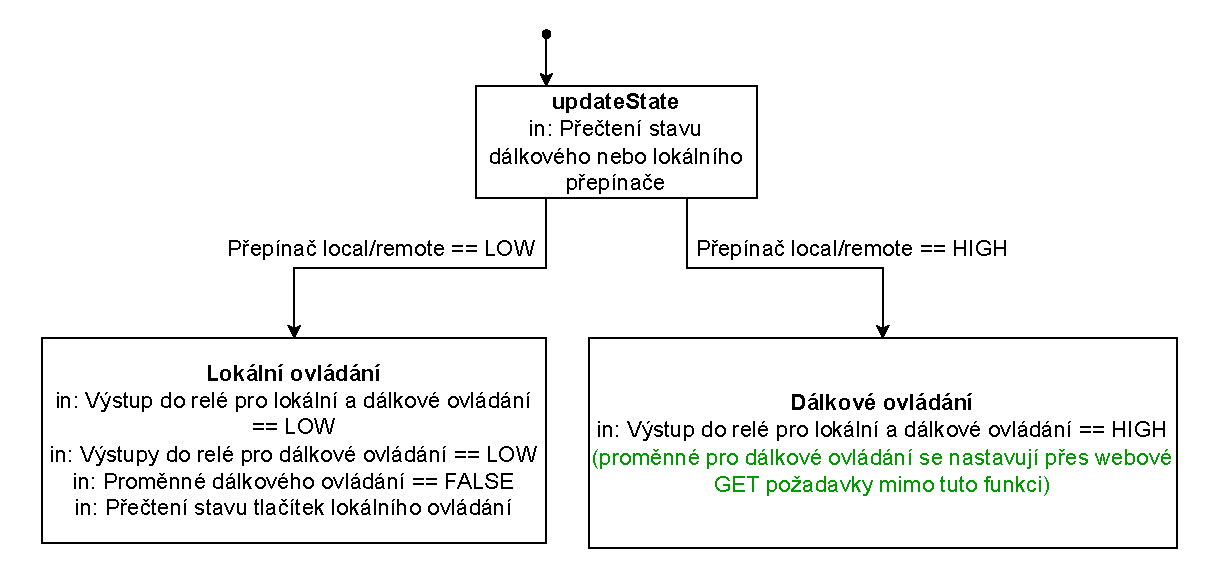
\includegraphics[width=1\linewidth]{images/StateFlow_Firmwaru_top.drawio.pdf}
	\caption{Začátek stavového diagramu}
	\label{fig:StateFlow_Firmwaru_top}
\end{figure}

Zde je vstup do stavového diagramu funkce updateState. Na začátku se přečte hodnota vstupního pinu vývojové desky ke kterému je připojený přepínač pro lokální nebo dálkové ovládání. Na základě této hodnoty se určí, jestli je systém ve stavu lokálního nebo dálkového ovládání. Podle této hodnoty se stavový diagram větví do diagramů pro lokální nebo dálkové ovládání.

\begin{figure}[H]
	\centering
	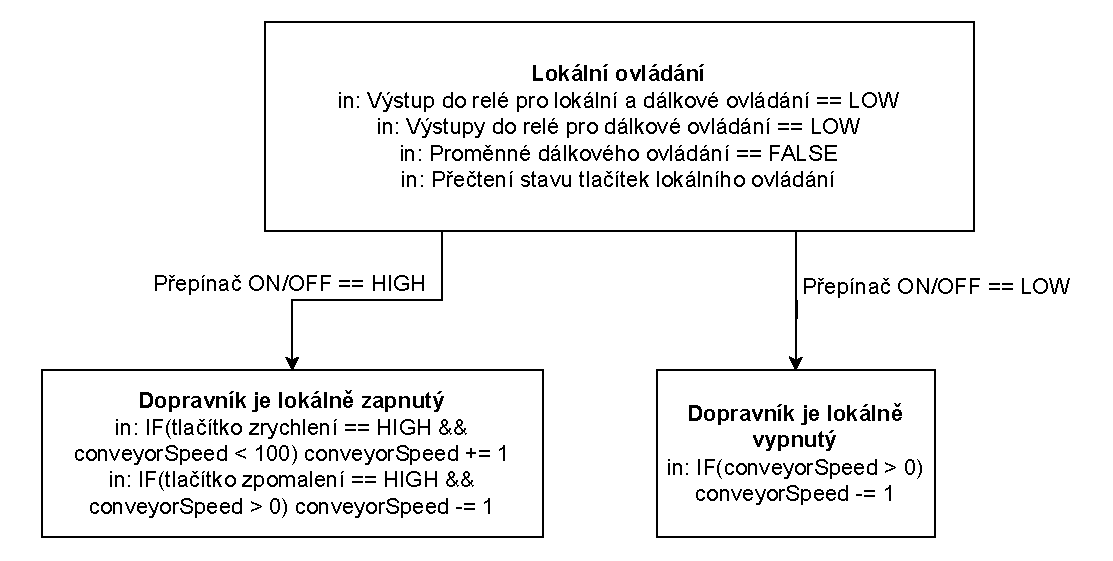
\includegraphics[width=1\linewidth]{images/StateFlow_Firmwaru_left.drawio.pdf}
	\caption{Strana stavového diagramu s lokálního ovládáním}
	\label{fig:StateFlow_Firmwaru_left}
\end{figure}

Ve stavu s lokálním ovládáním se nastaví výstupní pin vývojové desky ovládající tranzistor, který vypne relé, které přepíná mezi lokálním a dálkovým ovládáním. Následně se rovněž nastaví tranzistor ovládající dálkové ovládání, jelikož není potřeba toto relé mít zapnuté, když je tato větev obvodu deaktivována. Nakonec se nastaví proměnné dálkového ovládání na FALSE, aby byly vynulovány nastavené příkazy z WebServeru. Na konci provedení těchto bloků kódu se přečtou stavy tlačítek a přepínačů umístěných fyzicky na desce a na základě těchto stavů se pokračuje v provádění kódu.

V tomto stavu působí mikrokontroler spíše jako pouhý pozorovatel stavu tlačítek, než aby přímo spínal nějaké z relé. V blokovém schématu systému na obrázku \ref{fig:SchemaDesky} lze vidět, že tomu tak je protože je relé pro přepínání lokálního nebo dálkového ovládání připojené přímo k tlačítku, které bez žádného digitálního zpracování spíná nebo rozepíná 24V linku napětí pro ovládací panel. Toto vychází z požadavku na systém \textbf{Systém musí mít ovládání které je čistě analogové}.

Ze začátku se může pokračovat do větve \textbf{Dopravník je lokálně vypnutý}, a to v případě, že je hodnota přepínače, který lokálně ovládá stav ON/OFF, vyhodnocena LOW. V tomto stavu se pouze odečte hodnota rychlosti dopravníku, pokud je rychlost vyšší než 0 \footnote{rychlost dopravníku sledovaná v proměnné \texttt{conveyorSpeed} je pouze aproximace, která se zobrazuje v mobilní aplikaci a na LCD displeji. Není to vstup do ovládacího panelu.}.

Alternativně je možné pokračovat do větve \textbf{Dopravník je lokálně zapnutý}, pokud je hodnota přepínače ON/OFF vyhodnocena jako HIGH. V tomto případě se sleduje, jakým způsobem je dopravník ovládán, a na základě toho se přičte nebo odečte hodnota rychlosti dopravníku.

\begin{figure}[H]
	\centering
	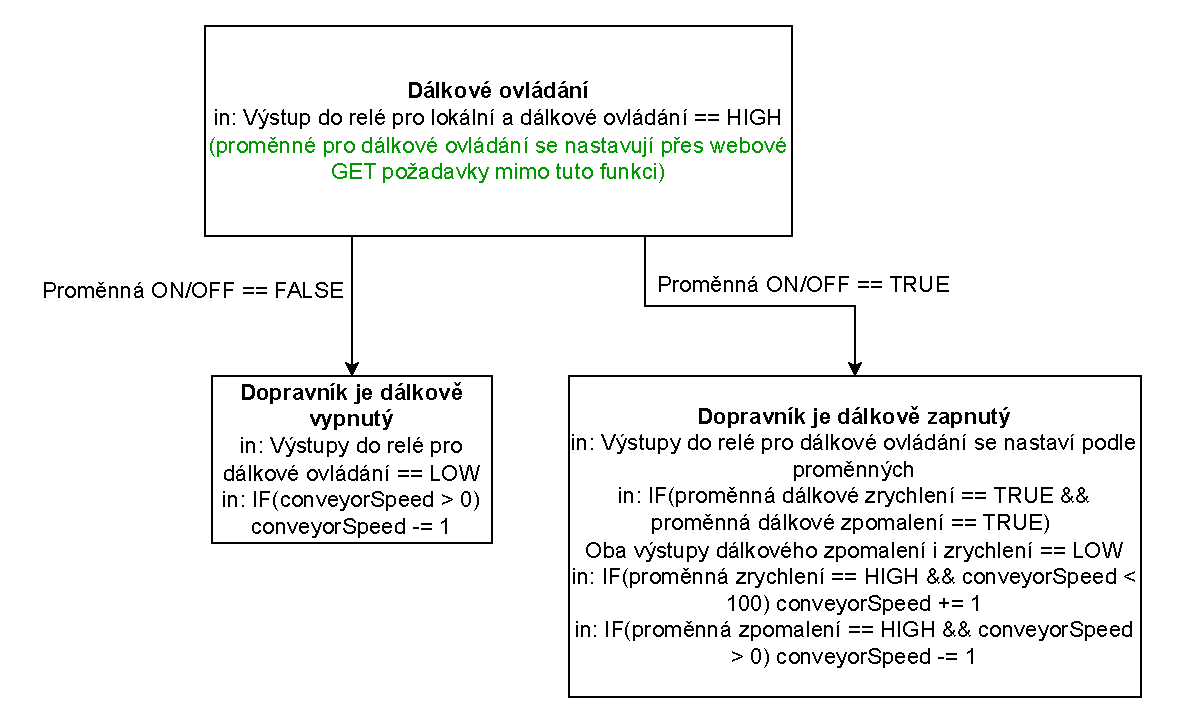
\includegraphics[width=1\linewidth]{images/StateFlow_Firmwaru_right.drawio.pdf}
	\caption{Strana stavového diagramu s dálkovým ovládáním}
	\label{fig:StateFlow_Firmwaru_right}
\end{figure}

Ve stavu s dálkovým ovládáním se nastaví výstupní pin, který ovládá relé pro dálkové nebo lokální ovládání, na úroveň HIGH. V rámci tohoto stavu už není nic dalšího provedeno, jelikož se proměnné, na základě kterých se ve stavovém diagramu pokračuje, nastaví při zpracování GET požadavků, které přicházejí na WebServer.

WebServer tedy nastavuje proměnné, na základě kterých se v tomto stavovém diagramu pokračuje v provádění kódu. Tyto proměnné jsou inicializovány na hodnotu FALSE, a proto se po přepnutí do režimu dálkového ovládání dopravník vypne. Během provádění stavového diagramu dálkového ovládání nejsou tyto hodnoty vynulovány, a je proto nutné přes WebServer nastavit proměnné jak na hodnotu TRUE, tak na hodnotu FALSE.

Pokud přes WebServer bude proměnná ON/OFF nastavena na hodnotu FALSE, poté se vypne relé, které ovládá dálkové ovládání, a sníží se hodnota rychlosti dopravníku až na 0.

Pokud se přes WebServer proměnná ON/OFF nastaví na hodnotu TRUE, sepne se tranzistor, který přivede proud do relé pro dálkové ovládání. Podobně se spustí relé, které zrychluje nebo zpomaluje dopravník přes ovládací panel, pokud jsou jejich specifické proměnné nastavené na hodnotu TRUE. Také zde se zvyšuje nebo snižuje hodnota aproximace rychlosti.

\subsubsection{Jak aplikace aproximuje rychlost dopravníku}\label{sec:AproximaceRychlostiDopravniku}
%\purpose{Vysvětlit jak se pomocí Tickeru aproximuje rychlost dopravníku}
V předchozí kapitole byla zmíněna proměnná \textit{conveyorSpeed} která si udržuje aproximovanou hodnotu rychlosti dopravníku. Aproximace rychlosti vychází z předpokladu, že frekvenční měnič zrychluje asynchronní motory dopravníku lineárně. Tento předpoklad je smysluplný, jelikož bývají frekvenční měniče v praxi často konfigurovány s lineárními rampami pro zrychlení a zpomalení ovládaných motorů. Tento předpoklad byl ověřen přímo na frekvenčním měniči v hale společnosti Honeywell a bylo tedy zkontrolováno, že platí.

Při testování bylo také zjištěno, že frekvenční měnič zrychluje o 500 otáček za 10 sekund. Zrychlení frekvenčního měniče je tedy $50ot/min$ za sekundu, což je z maximální hodnoty $1500ot/min$ (definovaná při nastavení ovládacího panelu v kapitole \ref{sec:NastaveniOvladacihoPanelu}) zrychlení $3.33\%/s$ neboli $1\%$ za $300ms$. Dopravník stejnou rychlostí i zrychluje i zpomaluje.

Samotná aproximace rychlosti dopravníků je tedy provedena tím způsobem, že se veřejná metoda \texttt{updateState} provádí každých $300ms$ a během každého provedení končí každá větev stavového diagramu aktualizací hodnoty \texttt{conveyorSpeed} Tato aktualizace je vždy provedena tím způsobem, aby hodnota patřila do intervalu $<0,100>\%$ z maximální rychlosti.

Volat funkci \texttt{updateState} každých $300ms$ by mělo být pro aproximaci dostatečně pravidelné. Jediný způsob jak by aproximace mohla nabývat špatných hodnot je pokud by byl systém ovládaný v lokálním režimu ovládání, tlačítko zrychlení by bylo sepnuté po dobu těsně menší než $300ms$ a zrovna tato doba vyšla na dobu mezi volání funkce \texttt{updateState}. Toto je chyba která může nastat obecně u jakéhokoliv vzorkování. Pokud by se tak stalo i opakovaně, stejně by byla chyba v řádu jednotek procent, což je zanedbatelné.

Naopak častější volání funkce \texttt{updateState} než $300ms$ by vyžadovalo vyšší spotřebu energie a bralo by to zbytečně výpočetní výkon vývojové desky, která ho spíše může využít pro odpovídání na webové požadavky co přichází na WebServer.

Způsob jakým je funkce \texttt{updateState} spuštěna každých $300ms$ je pomocí nastavení časovače skrz framework jménem \texttt{Ticker}. \texttt{Ticker} je open-source knihovna, která může být vložena do jakéhokoliv projektu založeném na Arduino framework. Zde je příklad kódu pro nastavení \texttt{Ticker} knihovny:

\begin{lstlisting}[language=C++, caption={Způsob používání \texttt{Ticker} knihovny}, label={lst:TickerKnihovnaExample}]
#include "Ticker.h"

void blink() {
	digitalWrite(LED_BUILTIN, ledState);
	ledState = !ledState;
}

void setup() {
	Ticker timer(blink, 500);
	timer.start();
}

void loop() {
	timer.update();
}
\end{lstlisting}

Používání \texttt{Ticker} knihovny tedy spočívá v tom, že si stačí zaobalit kód, který má být vykonáván, do samostatné callback funkce. Následně je možné vytvořit \texttt{Ticker} objekt ve kterém jsou vstupy tato callback funkce a čas který určuje jak často má být kód vykonáván. Pro kontrolu se doporučuje ještě přidat \texttt{update} metodu vytvořeného \texttt{Ticker} objektu do \texttt{loop} funkce.

Díky možnosti nastavit pomocí knihovny \texttt{Ticker} metodu \texttt{updateState} vzniká dobrý způsob jak dávat uživatelům systému vědět, jakou má dopravník aktuální rychlost i bez toho, aby bylo připojené zařízení Sinamics IOP-2 kterým se ovládací panel programuje (popsáno v kapitole \ref{sec:NastaveniOvladacihoPanelu}).

\section{Software v mobilní aplikaci}\label{sec:SoftwareVMobilniAplikaci}
% \purpose{V téhle sekci popíšu jak přesně funguje mobilní aplikace kterou jsem vytvořil a poznatky s tím spojené.}

Jak už bylo nastíněno v sekci \ref{sec:PopisFunkceSystemu}, primární důvod proč bylo rozhodnuto, že bude systém ovládaný přes mobilní aplikaci je, že není potřeba mít další zařízení, které bude fungovat jako dedikovaný hardwarový ovladač systému. Díky tomu je celkový systém přenositelnější a jednodušší ovládat, jelikož mobilní zařízení musí uživatelé mít už i kvůli zapisování dat z kontroly dopravníků. Komunikace mobilní aplikace a vývojové desky je realizována pomocí bezdrátové technologie WiFi, což umožňuje komunikaci v řádech desítek metrů (u nejnovějšího WiFi protokolu do 90 metrů).
\cite{DosahWIFIProtokolu}

Vzhledem k požadavku na systém s názvem \textbf{Uživatelská přívětivost systému} je navíc velmi výhodné mít systém ovládaný mobilní aplikací, jelikož je možné mít prakticky veškeré informace ohledně nastavování ovládacího panelu frekvenčního měniče na jednom místě. Tohle výrazně zlepšuje uživatelské používání systému, protože uživatelé nemusí hledat dokumentaci, když je na stejném místě jako ovládací prvky systému.

Mobilní aplikace není technicky vzato pro systém potřebná. WebServer je možné ovládat i přes webový prohlížeč. S takovým ovládáním by ale systém ztrácel další funkce, které mobilní aplikace nabízí. To je třeba zmiňovaná dokumentace uvnitř aplikace, nebo možnost mít automaticky aktualizovanou hodnotu rychlosti dopravníku a stavu ovládání. Velká výhoda aplikace je také ovládání více dopravníků najednou.

\subsection{Architektura aplikace}
%\purpose{Vysvětlit jakým způsobem jsem navrhoval architekturu aplikace a proč. Architektura = statická frontendová webová aplikace převedená do mobilní podoby pomocí WebView. Výhody jsou jednoduchost implementace GET requestů ve webové aplikaci. Zde taky přestavit React a Capacitor.}

Navržená mobilní aplikace vůbec není mobilní aplikace v tradičním slova smyslu, ale spíše jde o webovou aplikaci. Tuto webovou aplikace lze pomocí některých knihoven a rozšíření spolehlivě konvertovat do mobilní aplikace. Zde budou popsány důvody tohoto rozhodnutí.

Běžná webová aplikace má dvě hlavní části:

První část se jmenuje \textbf{front-end} a je to uživatelská část aplikace - obsahuje veškerý kód, který je prováděn u uživatele v prohlížeči. To většinou bývají jednodušší JavaScriptové bloky kódu, veškerá struktura a obsah aplikace (psaná v jazyce HTML) a veškeré formátování aplikace (běžné psané v jazyce CSS). Všechno ve front-end části jakékoliv webové aplikace je možné si dohledat pomocí rozhraní jako jsou \textbf{Chrome Developer Tools} (Více popsané v kapitole \ref{sec:DesignAplikace}), které umí kterémukoliv uživateli ukázat celý front-end kód webové aplikace.

Druhá hlavní část webové aplikace se jmenuje \textbf{back-end} a je to část aplikace kterou běžný uživatel nevidí. Obsahuje data seřazená v databázích, které je možné si pomocí různých příkazů načíst do front-end části. Také umí využívat server pro provádění různých výpočtů, které jsou buďto moc náročné, anebo musí být z určitých důvodů schované před běžnými uživateli.

Z hlediska softwarové architektury byla aplikace koncipována jako statická webová aplikace - tedy čistě front-endová aplikace bez back-end části. Aplikace byla postavená na knihovně jazyka JavaScript jménem \textbf{React}, což je dlouhodobě jedno z nejpopulárnějších rozhraní pro tvorbu webových aplikací (jak tvrdí studie nejpoužívanějších jazyků pro webové programování \cite{ReactWebDeveloperPopularity}). Specificky byla použita \textbf{Vite} verze Reactu, která je optimalizována pro rychlost aplikace.
\cite{ViteReactWeb}

Aby bylo možné programovat webové aplikace, je potřeba mít nainstalovanou aplikaci \textbf{Node.js}, která mimo jiné usnadňuje programování webové aplikace tím, že umí v reálném čase ukazovat jak každá změna React kódu ovlivnila aplikaci pomocí takzvaného "development" serveru, který je dostupný na lokální síti počítače, na kterém je node.js spuštěný.

Programování webové aplikace probíhalo tím způsobem, že se každá verze webové aplikace testovala tím způsobem, že se překonvertovala do statických souborů (obsahující pouze HTML, CSS a JS soubory) pomocí příkazu \texttt{vite build}. Ten přeloží syntax jazyka React do souborů, které jsou ekvivalentní, ale narozdíl od React syntaxu jim rozumí každý webový prohlížeč.

Když existuje tato "čistá" verze aplikace, je možné použít framework jménem \textbf{Capacitor}, který je vytvořený specificky pro to aby bylo možné ho pomocí node.js nainstalovat do knihoven pro webové programování jako je React. Následně je možné pomocí několika příkazů Capacitor frameworku přeložit tuto verzi aplikace do souborů mobilní aplikace.
\cite{CapacitorDocs}

Nakonec je možné si tuto složku konvertované mobilní aplikace otevřít v prostředí \textbf{Android Studio} a tam si z daného projektu vytvořit soubor o příponě \texttt{.apk}, který si umí nainstalovat každé android zařízení. Pomocí capacitor je možné konvertovat i do mobilní aplikace pro zařízení firmy Apple. Na konvertování do instalačního souboru je ale potřebné mít i stolní počítač značky Apple, kde je možné aplikaci konvertovat pomocí \textbf{Xcode}.

\subsubsection{Proč webová aplikace?}\label{sec:ProcWebovaAplikace}
Důvod, proč byla mobilní aplikace programována jako webová a ne přímo mobilní, je ten, že jejím hlavním účelem je posílat GET požadavky na IP adresu vývojové desky. Na tento úkol jsou moderní webové aplikace velmi dobře optimalizovány.

Každá větší webová aplikace dostupná na internetu má front-end část a v jejím rámci posílá webové požadavky na svůj server, kde je spuštěn back-end aplikace. Tyto požadavky souvisejí s dynamickým obsahem, který může být:
\begin{itemize}
	\item Načtení reklamy na sociální síti.
	\item Potvrzení objednávky na e-shopu.
	\item Provádění náročnějších kalkulací pomocí výkonu co poskytuje server.
	\item A další.
\end{itemize}

V případě navrženého systému sice nemá mobilní aplikace vlastní back-end server, ale zato má WebServer hostovaný na mikrokontroleru. Ten přijímá příkazy jako "zrychlit dopravník" a naopak vysílá informace jako rychlost dopravníku.

Z těchto důvodů je mnohem snazší navrhnout nejdříve webovou aplikaci, implementovat komunikaci obou částí webového systému a následně webovou aplikaci konvertovat do mobilní. Pokud by byla mobilní aplikace programovaná od základu pomocí knihoven pro tvorbu mobilních aplikací, zmizel by sice snadno řešitelný problém konverze webové aplikace do mobilní, ale vznikl by problém implementace webové komunikace uvnitř mobilní aplikace.

\subsubsection{Adresy webové aplikace}\label{sec:AdresyWeboveAplikace}

Webová aplikace má tři URL adresy:
\begin{itemize}
	\item \textbf{Vstupní stránka (adresa "/")} – Tato stránka obsahuje hlavní část aplikace, která umožňuje ovládání dopravníků.
	\item \textbf{Setup (adresa "/setup")} – Tato stránka obsahuje návod, jak dopravník nastavit, aby s tímto zařízením správně fungoval.
	\item \textbf{Help (adresa "/help")} – Tato stránka obsahuje popis častých chyb, které mohou nastat při používání zařízení a při nastavování dopravníků, a rady k jejich vyřešení.
\end{itemize}

Tyto URL adresy zůstávají stejné i při převedení do mobilní aplikace. Je ovšem potřeba mít v aplikaci nějaký způsob, jak se pomocí tlačítek mezi těmito adresami navigovat, protože při převedení webové aplikace do mobilní chybí adresní řádek, kde by bylo možné tyto adresy zadat. Tuto navigaci v mobilní aplikaci zajišťuje hlavička s navigačním panelem, která obsahuje tyto odkazy.

%Tohle nepřidávám, protože si myslím že není třeba zdlouhavě popisovat jak funguje React uvnitř praktické části.
%\purpose{Co je to React a proč se hodí na návrh této webové aplikace. Co je to HTML, CSS a JS. Co je to reaktivnost komponentů. Jak se react využívá. Možná sem přidat co je to tailwind a Lucide for React.}
%React je web developmentovej framework a hodí se na návrh, protože přes node package manager už existují frameworky, který mi umožní webový aplikace portovat do mobilní aplikace - tenhle framework se jmenuje capacitor. Capacitor používá WebView (pro Android) nebo WKWebView (pro iOS) a díky tomu umožňuje zobrazit si webové aplikace na zařízení.\cite{CapacitorDocumentationFAQ}
%Webovou aplikaci navrhuji, protože to, co chci aby dělala je aby jenom posílala GET požadavků na IP adresu mikrokontrolleru kterou hostuje NodeMCU, což je hodně jednoduchá věc na implementaci ve webové aplikaci.
%\source{React může mít zase jako zdroj nějakou odbornou literaturu zaměřenou na react (pokud něco takového najdu) anebo online dokumentaci.}

\subsection{Použité knihovny a technologie v aplikaci}
% \purpose{Vysvětlit co za frameworky (knihovny) jsem při developování aplikace použil aby to fungovalo co nejlépe}
Při programování webové aplikace bylo použito několik knihoven, které webovým developerům pomáhají při návrhu aplikací. Zde je krátký popis každé z těchto technologií a role, jakou zastaly při programování webové aplikace.

\subsubsection{HTML, CSS a JS}
HyperText Markup Language neboli HTML je jeden z prvních jazyků, které stály u zrodu internetu. Definuje strukturu webových stránek a obsahuje veškerý text. Dále je zde Cascading Style Sheets neboli CSS, které popisuje vzhled dokumentu napsaného v HTML. JavaScript neboli JS je odlehčený programovací jazyk s just-in-time kompilací, který je nejvíce známý tím, že dodává funkčnost webovým stránkám. Je to ale i skriptovací jazyk pro aplikace mimo webové prostředí, jako například Node.js nebo Adobe Acrobat.
\cite{HTMLweb, CSSweb, JSweb}

Tyto technologie jsou stále využívány na této webové stránce, ačkoli se v nich přímo neprogramovalo. Tyto programovací jazyky jsou základní stavební kameny prohlížeče, a proto je nutné každou aplikaci konvertovat do souborů těchto tří jazyků. Bez toho by nebylo možné zobrazit webovou stránku jak ve webové aplikaci, tak v mobilní aplikaci.

\subsubsection{React}\label{sec:React}
React je knihovna pro webový front-end založená na komponentech. Uvnitř těchto komponent je možné vkládat i HTML, což umožňuje spojit funkcionalitu s textem a strukturou.

React si zakládá na interaktivitě a reaktivnosti. U statických webových stránek, které jsou napsané přímo v HTML, CSS a JS, se jakákoliv změna projeví tím, že se musí znovu načíst celá stránka. Na druhou stranu React umí aktualizovat pouze ty části webové stránky, kde změna proběhla. Tomuto se říká reaktivnost webové stránky.
\cite{ReactWeb}

\subsubsection{TypeScript}
TypeScript je nadstavba JavaScriptu, která řeší jeho nedostatky. JavaScript například nemá implementovanou silnou typovou kontrolu, a tak je možné jakékoliv proměnné přiřadit jakoukoliv hodnotu. To může vytvářet chyby v kódu i přesto, že editor při psaní kódu žádnou chybu přímo neoznačil.

TypeScript je navíc vždy možné kompilovat do JavaScriptu, který je spustitelný v prohlížeči, a proto je velmi užitečný nástroj při programování složitějších aplikací.
\cite{TSweb}

\subsubsection{Tailwind}
Tailwind umožňuje developerům webových aplikací definovat vzhled prvků přímo v HTML kódu, čímž odpadá potřeba samostatných souborů se styly, jako je běžné u CSS.
\cite{Tailwindweb}

\subsubsection{DaisyUI}\label{sec:DaisyUI}
DaisyUI přidává speciální klíčová slova pro rozšíření knihovny Tailwind. Zatímco Tailwind poskytuje většinou specifická klíčová slova, která zpravidla přímo odpovídají jednotlivým vlastnostem CSS, DaisyUI funguje jinak. Tato knihovna umožňuje pod jedním klíčovým slovem sdružit více tailwind stylů.
\cite{daisyuiweb}

Díky tomu DaisyUI poskytuje styly pro celé komponenty, jako jsou například tlačítka nebo alert boxy. Také poskytuje ovládání motivu celé webové stránky, díky čemuž je s trochou konfigurace možné jednoduše měnit celkový vzhled stránky.

\subsubsection{Lucide for React}
Poslední použitou knihovnou je Lucide, knihovna ikon vytvořená pro React. V běžné webové stránce by vložení ikony, jako například koš pro odstranění dopravníku, vyžadovalo stažení souboru s příponou například \texttt{.svg} a jeho následnou úpravu a vložení do stránky.

S Lucide však stačí pouze použít předpřipravené React komponenty, které obsahují většinu často používaných ikon.
\cite{lucideWeb}

\subsection{Princip komunikace s WebServery}\label{sec:PrincipKomunikaceSeServery}
%\purpose{Co je to GET požadavek a jak se dá implementovat v JavaScriptu.}

Jak bylo nastíněno v kapitole \ref{sec:ProcWebovaAplikace}, způsob, kterým spolu komunikují mobilní aplikace a ESP8266 WebServer, spočívá ve využití webových GET požadavků.

GET požadavek je základní nástroj pro komunikaci mezi klienty a servery webové infrastruktury. Například při zadání URL adresy webové stránky do prohlížeče odešle prohlížeč GET požadavek na server nacházející se na dané webové adrese. Server tento požadavek zaregistruje a odpoví zasláním obsahu webové stránky (front-endu).

Přesně tímto způsobem komunikuje i mobilní aplikace s WebServerem běžícím na vývojové desce. Protože je vývojová deska připojena k hotspotu hostovanému mobilním zařízením s aplikací, může mobilní aplikace komunikovat s WebServerem jako s jakýmkoliv jiným serverem, a proto může podávat požadavky na různé adresy. Nastavení vývojové desky navíc umožňuje spustit různé bloky kódu po přijetí těchto GET požadavků.

V JavaScriptu se GET požadavky implementují tímto způsobem:
\cite{JavaScriptGET}

\begin{lstlisting}[language=JavaScript, caption={Základní způsob posílání GET požadavků v JavaScriptu }, label={lst:JavaScriptFetchFunkce}]
	async function getData() {
		const url = "https://example.org/products.json";
		try {
			const response = await fetch(url);
			if (!response.ok) {
				throw new Error(`Response status: ${response.status}`);
			}
			const json = await response.json();
			console.log(json);
		} catch (error) {
			console.error(error.message);
		}
	}
\end{lstlisting}

Níže jsou popsány tři hlavní způsoby využití GET požadavků pro ovládání systému:

\subsubsection{Jak dálkově spouštět dopravník}
V mobilní aplikaci je možné mít tlačítko, na něž lze kliknout, čímž se odešle GET požadavek na adresu \texttt{192.168.0.144/conveyorOn}\footnote{\texttt{192.168.0.144} je náhodně přiřazená lokální IP adresa mikrokontroleru, která se s každou vývojovou deskou mění.}. Po kliknutí na tlačítko vývojová deska zaregistruje tento požadavek a provede kód definovaný ve třídě \texttt{ConveyorController} (v kapitole \ref{sec:ConveyorController}). Tento kód nastaví proměnnou, na jejímž základě v další iteraci metody \texttt{updateState} dojde k sepnutí relé na desce plošných spojů, čímž se na ovládací panel frekvenčního měniče nastaví vysoká logická hodnota pro spuštění dopravníku.

\subsubsection{Jak získat data o rychlosti dopravníku}
Další možností je periodické vysílání GET požadavku funkcí. GET požadavky se zasílají na \texttt{192.168.0.144/getData}. Vývojová deska tento požadavek zaregistruje a odešle zpět odpověď ve formátu JSON. Tento přijatý soubor obsahuje informace o rychlosti dopravníku (v procentech) a o stavu ovládání (lokální nebo dálkové). Data v tomto formátu lze ve webových aplikacích snadno konvertovat do TypeScript objektu, který lze zobrazit v HTML kódu mobilní aplikace.

Pokud by React nebyl reaktivní (jak bylo vysvětleno v kapitole \ref{sec:React}), pak by se s každým přijetím dat musela celá webová stránka obnovit. S využitím funkce React knihovny lze však aktualizovat pouze rychlostní a ovládací data na stránce.

\subsubsection{Jak ovládat vývojovou desku bez mobilní aplikace}\label{sec:JakOvladatBezMobilniAplikace}
Nakonec není ani nutné používat mobilní aplikaci, ale stačí použít webový prohlížeč v mobilním telefonu k ovládání desky. V tom případě lze do URL adresy zadat \texttt{192.168.0.144/} bez další cesty. WebServer zde znovu zaregistruje požadavek a tentokrát odešle zpět HTML kód webové stránky, která je nakonfigurována jako hlavní odpověď ve třídě \texttt{ConveyorController}.

Tato webová stránka umožňuje ovládat vývojovou desku pomocí tlačítek, jež jsou nakonfigurována k odesílání GET požadavků na příslušné adresy vývojové desky. Tato stránka ovšem není reaktivní, protože se jedná o statickou HTML stránku. Kvůli tomu se aktuální hodnoty rychlosti a stavu ovládání zobrazí pouze po jejím načtení. Na obrázku \ref{fig:WebServerLandingPage} je zobrazen vzhled této webové stránky.

\begin{figure}[hptb]
	\centering
	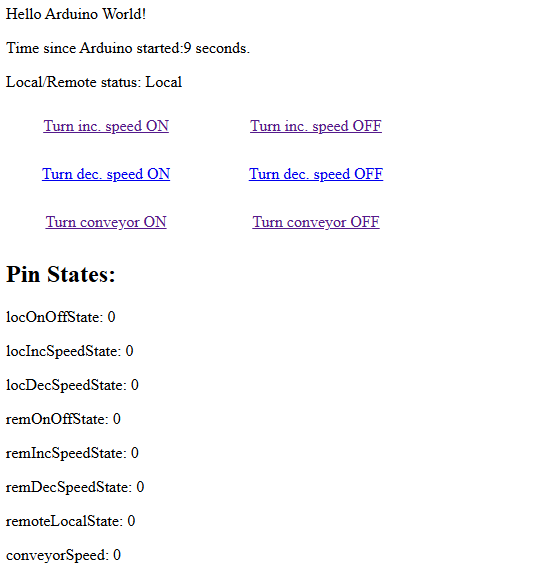
\includegraphics[width=0.6\linewidth]{images/WebServerLandingPage.png}
	\caption{Ukázka stránky pro ovládání vývojové desky bez mobilní aplikace}
	\label{fig:WebServerLandingPage}
\end{figure}

\subsection{Implementování GET požadavků s Capacitor}
%\purpose{Vysvětlit proč normální GET requesty nefungují (Omezení z WebView) a jak je tedy implementovat. Taky zmínit že jsou implementované ve funkci sendCommand.}

GET požadavky není kvůli konverzi webové aplikace do mobilní pomocí Capacitoru možné posílat běžným způsobem. Je tomu tak, protože v prostředí Android aplikace funkce \texttt{fetch} nefunguje stejně jako v prostředí webového prohlížeče. Tento problém je však již vyřešen komunitou Capacitoru, která pro tento účel vyvinula balíček s názvem CapacitorHttp. Tento balíček zjednodušuje posílání GET požadavků v rámci Capacitor aplikací tím, že poskytuje vlastní metodu GET, která má mírně odlišnou syntaxi upravenou tak, aby fungovala v mobilním prostředí WebView (konverze do mobilní aplikace je popsána v kapitole \ref{sec:KonvertovaniWeboveAplikaceDoMobilni}).

GET požadavky se v aplikaci používají tímto způsobem:
\begin{lstlisting}[language=JavaScript, caption={Rozšířený způsob posílání GET požadavků pro Capacitor mobilní aplikace}, label={lst:SendCommandFunkce}]
    // pred zacatkem komponentu:
    import { CapacitorHttp } from "@capacitor/core";
    import { HttpOptions } from "@capacitor/core/types/core-plugins";

    // uvnitr komponentu se strankou aplikace:

      // Posilani prikazu specifickemu dopravniku
  const sendCommand = async (ip: string, command: string) => {
    try {
      const options: HttpOptions = {
        url: `http://${ip}/${command}`,
      };

      const response: any = await fetchWithTimeout(
        CapacitorHttp.get(options),
        3000 // Nastaveni rychleho selhani pokud neni ziskana odpoved
      );

      setErrorMessage(null);
      console.log(response);
      try {
        const responseData = await response.json();
        console.log("Response data:", responseData);
      } catch (error: any) {}
    } catch (error: any) {
      console.error("Command failed:", error);
      setErrorMessage(`Command failed for ${ip}: ${error.message}`);

      // Kdyz selze odpoved tak se ihned nastavi dopravnik jako nedostupny
      setConveyors((prevConveyors) =>
        prevConveyors.map((conv) =>
          conv.ip === ip ? { ...conv, isOnline: false } : conv
        )
      );
    }
\end{lstlisting}
Nejdříve je nutné si importovat \texttt{HttpOptions} a \texttt{CapacitorHttp} z nainstalované Reactové Capacitor knihovny. Následně pokračuje definice komponentu, který obsahuje celou vstupní stránku aplikace a který je v rámci React aplikace zobrazován. Uvnitř stránky aplikace je definována funkce \texttt{sendCommand}.

Funkce \texttt{sendCommand} má jako vstupy IP adresu vývojové desky a adresu, na kterou bude posílat GET požadavek. Princip je takový, že se do \texttt{HttpOptions} nastaví jako URL celá IP adresa i s adresou požadavku a aplikace se poté pomocí funkce \texttt{CapacitorHttp.get} pokusí odeslat požadavek. Pokud byl požadavek úspěšně doručen, aplikace se bude pokoušet parsovat odpověď jako JSON. To se pro většinu odpovědí nezdaří, jelikož aplikace v rámci některých odpovědí zasílá i HTML kód, aby bylo možné ji ovládat i přes webový prohlížeč (popsáno v kapitole \ref{sec:JakOvladatBezMobilniAplikace}). Pokud se ale nepodaří parsovat odpověď, nijak to neovlivňuje funkčnost aplikace a je tak přijatelné mít řádek pro parsování odpovědi jako JSON ve try-catch bloku, který případnou chybu potlačí.

Pokud \texttt{sendCommand} nezíská odpověď do 3 sekund, kód aplikace pomocí funkce \texttt{fetchWithTimeout} signalizuje chybu, která se zobrazí v uživatelském rozhraní. Toto je obzvlášť důležitá funkce, protože se tato chyba uživateli v aplikaci ukáže, pokud během 3 sekund webový server neodpoví na požadavek. To se může stát hlavně pokud uživatel opustí dosah, ve kterém je webový server schopen komunikovat, a má tak jasnou vizuální indikaci, že by se pro ovládání dopravníku měl přiblížit. Tato implementace také vypíná možnost stisknout tlačítka, která ovládají dopravník, jelikož by na ně vývojová deska nereagovala.

% Tahle část mi přijde, že opakuje předešlé body, nepřidává nic moc navíc a ani nevím jak bych ji pojmenoval :D. Takže je asi tento generickej popis jak funguje aplikace zbytečnej, když to mám cca popsaný v ostatních kapitolách. Navíc nemá smysl vysvětlovat jak funguje aplikace bez toho abych vysvětloval jak funguje React - a to by bylo už moc textu pro tuhle práci.
%\subsection{Funkčnost aplikace (hodně stran)}
%\purpose{Tady už vůbec neřešit jak ta aplikace vypadá, ale zaměřit se na to co ta aplikace dokáže a jak to dělá. Struktura hlavní stránky, správa seznamu dopravníků, ovládání dopravníků je zahrnuto v sendCommand, získávání a zobrazování stavu skrz sendCommand a stránky Setup a Help. TOHLE BUDE HLAVNÍ MEAT TÉHLE KAPITOLY}
%
%Základ hlavní stránky je využívání reaktivnosti Reactu. Jelikož je aplikace dělaná v Reactu, je možné plynule přidávat dopravníky do seznamu bez toho aby se aplikace musela načítat pořád znovu. React nám také dává možnost ukládat IP adresy dopravníků do lokální paměti stránky a tak si aplikace vždy při spuštění načte data o dopravnících, které v aplikaci byly při posledním ukončení. React také umožňuje veškeré další funkce jako implementace GET požadavků a na základě těchto GET požadavků upravovat vzhled aplikace - jako například, že pokud GET požadavek nedostane úspěšnou odpověď do tří sekund, aplikace vyhodnotí daný nodeMCU server jako nefunkční a na základě toho uživatele vizuálně upozorní a vypne možnost se pokoušet o spojení s zařízením.
%
%\subsubsection{Co funkci sendCommand používá}
%\purpose{Vysvětlit proč je funkce sendCommand tak důležitá}
%
%Funkci sendCommand používají všechny tlačítka aplikace, které je možné vidět na obrázku \ref{fig:MobilniAppScreenshots} (tlačítka ON/OFF, zrychlení a zpomalení dopravníku).
%
%Funkce sendCommand se ale navíc sama provádí každé 2 sekundy pro každý dopravník přidaný do vstupní stránky aplikace. Provádí se tam GET požadavek na adresu /getData na adrese každého nodeMCU serveru. Tato adresa odpovídá s aktuální (aproximovanou) rychlostí dopravníku a s aktuálním stavem jestli je dopravník ovládaný lokálně nebo dálkově. Tato adresa už odpovídá pouze json souborem a díky tomu je důležité se i v rámci sendCommand pokoušet o přeložení odpovědi do javascript objektu pomocí příkazu $response.json()$. V případě těchto požadavků už program neselže s chybou a díky tomu uživatelské rozhraní aplikace získává informaci o rychlosti a stavu dopravníků, kterou může zobrazovat ve vstupní stránce jak je vidět na obrázku \ref{fig:MobilniAppScreenshots}.

\subsection{Design aplikace}\label{sec:DesignAplikace}
% \purpose{Zde vysvětlit jak jsem postupoval při designování aplikace. Vysvětlit co je to header aplikace a že mám nějakej styling kterej je pro každý React komponenty aplikovanej automaticky.}

Tato mobilní aplikace sice byla naprogramována jako webová, ale její design byl od začátku koncipován s ohledem na optimální vzhled při používání na mobilních zařízeních. Jelikož je v dnešní době kladen velký důraz na to, aby i webové stránky vypadaly dobře na mobilních zařízeních, existují pro tento účel nástroje, jako jsou Chrome Developer Tools.

\textbf{Chrome Developer Tools} je soubor nástrojů pro webové vývojáře dostupný pro každého uživatele prohlížeče Google Chrome. V rámci těchto nástrojů je možné změnit vzhled webové stránky na jakékoli rozlišení za účelem testování vzhledu na tabletech a mobilních zařízeních různých velikostí. Chrome Developer Tools však kromě této funkce obsahuje i velké množství dalších užitečných nástrojů pro webové vývojáře, jako například konzole (kde se zobrazují chybové zprávy), nástroje pro analýzu rychlosti aplikace, náhled celého HTML kódu a mnoho dalších.

Všechny barvy aplikace jsou definovány pomocí klíčových slov v rámci správy motivů poskytované knihovnou DaisyUI (rozšíření, krátce představeného v kapitole \ref{sec:DaisyUI}). Tato klíčová slova jsou například \texttt{base, primary, secondary, accent} a další. Nastavení aplikace tímto způsobem dává možnost parametrizace barev, jelikož se určuje spíše účel barvy než její přímá hodnota. Díky tomuto nastavení je možné měnit motiv stránky na jeden z 30 přednastavených motivů od DaisyUI, nebo si nastavit vlastní barvy. Navíc je možné nastavit různé motivy pro světlé i temné rozhraní mobilního zařízení. V \cite{DaisyUIthemeGenerator} lze vidět, jaká všechna nastavení DaisyUI poskytuje v rámci správy motivů.

V obrázku \ref{fig:LandingPageAnnotated} je zobrazen vzhled hlavní stránky aplikace pro světlé rozhraní telefonu.

\begin{figure}[hptb]
	\centering
	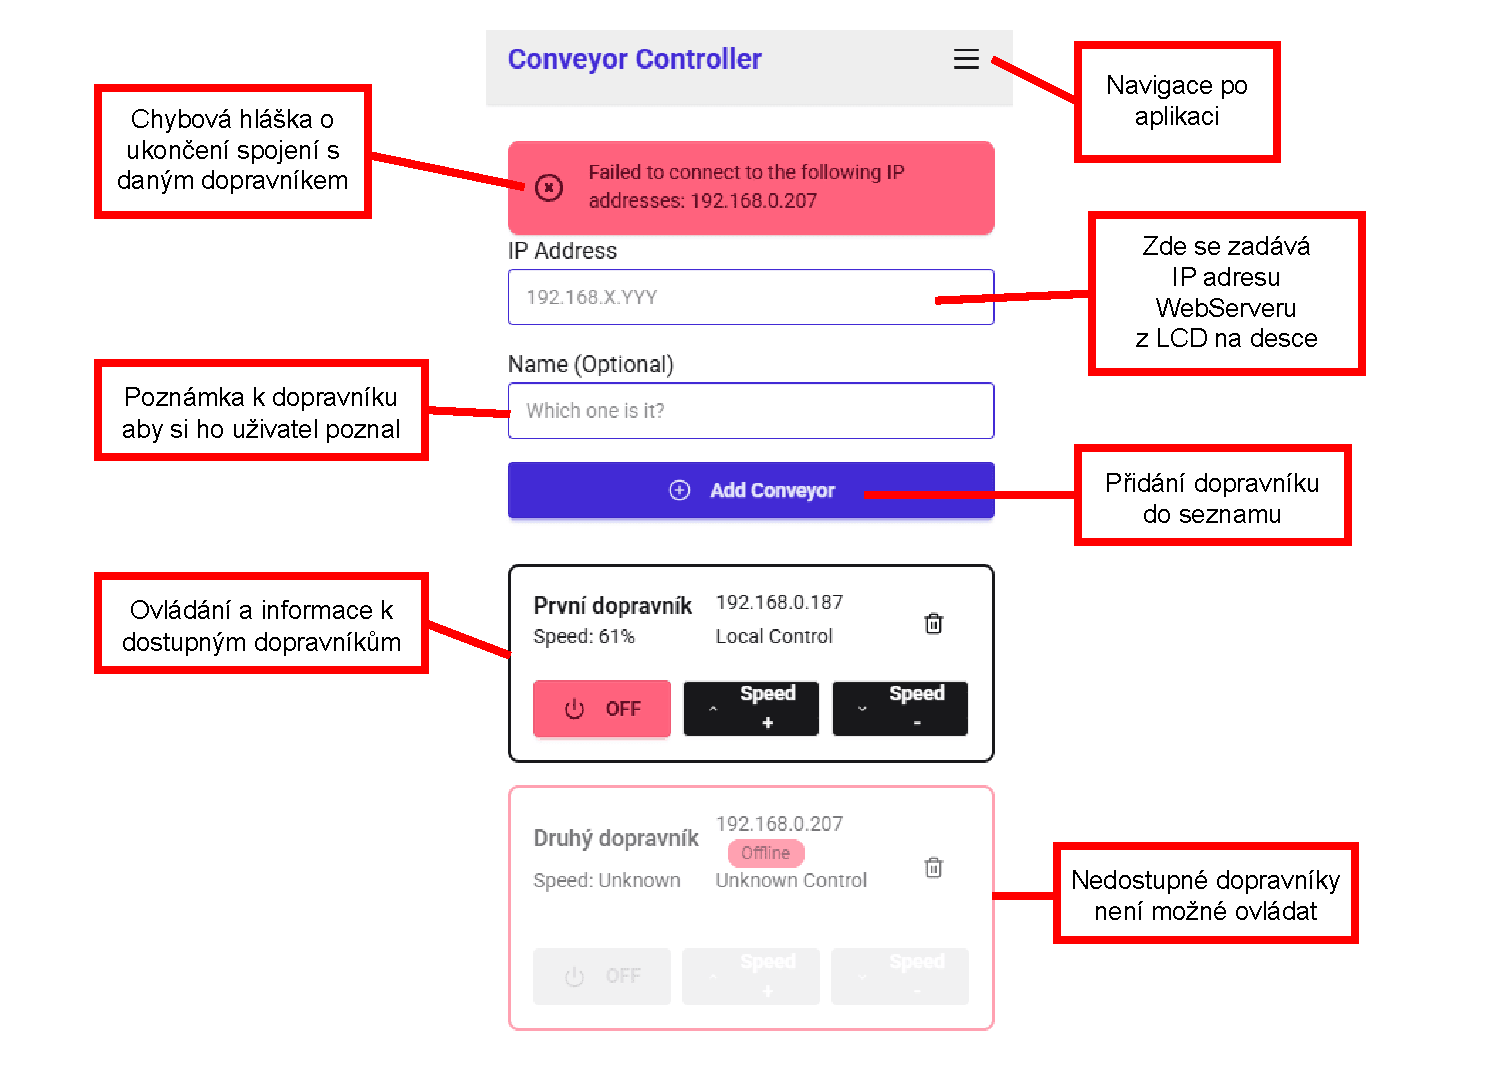
\includegraphics[width=1\linewidth]{images/LandingPage_Annot.drawio.pdf}
	\caption{Popis designu hlavní stránky aplikace}
	\label{fig:LandingPageAnnotated}
\end{figure}

Tento obrázek aplikace byl pořízen na počítači v rozhraní Chrome Developer Tools. Na hlavní stránce aplikace lze nahoře vidět hlavičku, která obsahuje tlačítko navigace. Po stisknutí tohoto tlačítka se zobrazí odkazy na další stránky obsažené v aplikaci, jak bylo popsáno v kapitole \ref{sec:AdresyWeboveAplikace}. Lze také vidět chybovou zprávu, která se však zobrazí pouze v případě, že se nepodařilo spojit s některým webovým serverem.

Uprostřed stránky je následně vidět část aplikace určenou k přidávání IP adres vývojových desek, čímž se v dolní části aplikace vytvoří rozhraní pro jejich ovládání. Zde je možné zadat IP adresu desky tak, jak je napsaná na LCD displeji fyzické desky připojené k dopravníku. Dále je zde poznámka, která je v aplikaci pouze pro identifikaci dopravníku a na funkci nemá žádný vliv. Po stisknutí tlačítka pro přidání dopravníku se přidají informace o dopravníku do matice objektů obsahující všechny dopravníky.

V dolní části aplikace je pak oblast obsahující tlačítka pro ovládání takto přidaných dopravníků. Jak bylo popsáno v kapitole \ref{sec:PrincipKomunikaceSeServery}, tato tlačítka jsou nastavena pro posílání GET požadavků na adresy vývojové desky. Na jakou adresu se požadavek odešle, záleží na tom, zda již bylo tlačítko stisknuto. Například pokud dopravník nebyl ještě spuštěn pomocí aplikace, tlačítko \texttt{ON/OFF} bude ve stavu \texttt{OFF}, bude mít červenou barvu a bude posílat GET požadavek na adresu "/conveyorOn". Po stisknutí se okamžitě změní jeho stav na \texttt{ON}, bude mít zelenou barvu a bude posílat GET požadavek na adresu "/conveyorOff". V aplikaci je pro tyto účely implementována lokální paměť a při zavření se ukládá, které dopravníky byly dostupné a jak byly ovládány.

\subsection{Konvertování webové aplikace do mobilní aplikace}\label{sec:KonvertovaniWeboveAplikaceDoMobilni}
% \purpose{Zmínit že je možné react aplikaci pomocí Android Studia portnout do .apk souboru který používá WebView a dále co je to CORS a že operační systém androidu defaultně zakazuje HTTP requesty.}

Aplikace byla konvertována v základní verzi programu \textbf{Android Studio} verze 2024.3.1 a pro konverzi nebylo potřeba instalovat žádné další balíčky.

Způsob konverze React aplikace do její mobilní podoby spočívá v zapouzdření webového obsahu do nativní komponenty. V případě zařízení s Androidem se k tomu využívá \textbf{WebView}, který zobrazuje webový obsah v simulovaném webovém prohlížeči, a díky tomu je možné některé funkce webové aplikace přímo integrovat do mobilní verze, zatímco některé funkce (jako třeba zasílání GET požadavků) je možné implementovat pomocí knihoven Capacitoru, jelikož v původní syntaxi ve WebView nefungují.
\cite{CapacitorHowItWorks}

Před samotným zapouzdřením aplikace je potřeba aplikaci připravit do tzv. "produkční verze". Pro vytvoření této verze stačí v moderních JavaScriptových knihovnách, jako je React, zkompilovat zdrojový kód. Výsledkem této konverze jsou statické soubory HTML, CSS a JS.

Aby bylo možné úspěšně komunikovat s webovými servery, je nutné splnit některé bezpečnostní aspekty v případech, kdy web komunikuje se serverem, specificky mechanismus \textbf{Cross-Origin Resource Sharing} neboli CORS. To je protokol, který pro servery z bezpečnostních důvodů omezuje, která zařízení mají právo na tento server zasílat požadavky, jako je GET požadavek. Mobilní aplikace je jiné zařízení než webový server a je na jiné lokální IP adrese, a tak je potřeba tento bezpečnostní aspekt vyřešit, jinak spolu nebudou moct tato dvě zařízení komunikovat. To bylo nakonec vyřešeno tak, že jsou na každé webové adrese webového serveru nastaveny CORS hlavičky v HTML kódu tak, aby přijímal jakékoli GET požadavky z jakékoli IP adresy. Toto rozhodnutí bylo provedeno, jelikož mobilní zařízení může mít jakoukoli IP adresu na lokální síti. Tímto způsobem je ale komunikace stále bezpečná, jelikož webový server je dostupný pouze lokálně, a tak by na něj mohl být útok proveden pouze v případě, že by byl útočník také připojen k hotspotu mobilního zařízení.
\cite{CORShowItWorks}

Dalším důležitým aspektem specifickým pro platformu Android je výchozí konfigurace síťové bezpečnosti. U novějších verzí Androidu už operační systém standardně zakazuje komunikaci pomocí nešifrovaného protokolu HTTP a preferuje zabezpečený protokol HTTPS. Jelikož webový server v této implementaci využívá pro komunikaci nešifrovaný protokol HTTP, bylo nutné tuto restrikci obejít. Povolení komunikace přes HTTP bylo provedeno pro všechny lokální domény modifikací konfiguračního souboru \texttt{AndroidManifest.xml} mobilní aplikace, který je generován při konverzi pomocí Capacitoru. Zavedení protokolu HTTPS na webovém serveru by v kontextu lokální sítě nepřineslo žádné bezpečnostní benefity.
\cite{cleartextTraffic}

Výsledkem konverze aplikace je spustitelný soubor ve formátu \texttt{.apk}, který lze nainstalovat na mobilních zařízeních s Androidem. Konverzi je možné provést bez certifikace pro distribuci přes Google Play Store, ale v takovém případě se na zařízení zobrazuje jako "neověřená". V rámci testování ale aplikace prošla úspěšně standardní virovou kontrolou Google Play, což potvrdilo, že během procesu konverze v aplikaci nepřibyl žádný virus. Vzhledem k tomu, že je aplikace určená pro interní použití v rámci společnosti Honeywell a nebude veřejně distribuována, není zapotřebí provádět kroky nezbytné pro publikaci v Google Play Storu.

\subsubsection{Postup konvertování webové aplikace}
% \purpose{Už nepsat teorii jak by se dala aplikace zkonvertovat jako ve kapitole \ref{sec:KonvertovaniWeboveAplikaceDoMobilni} ale specificky napsat jak jsem postupoval při konvertování aplikace krok za krokem.}

Pro konvertování je potřeba mít nainstalované Android Studio a Node.js. Dále musí být inicializována React aplikace a v ní nainstalovaný a nastavený Capacitor. Složka webové aplikace by měla být vzhledem k Android Studiu mimo složky s českou diakritikou a mimo složky synchronizované pomocí cloudových aplikací.

Specifický postup konvertování webové aplikace do mobilní je následující:

\begin{enumerate}
	\item Začíná se v nejnovější verzi React webové aplikace.
	\item Sestavení do "produkční verze webové aplikace" se provádí pomocí příkazu \texttt{npm run build}.
	\item Dále je potřeba aplikaci synchronizovat s Capacitorem pomocí příkazu \texttt{npx cap sync}.
	\item Nyní je potřeba otevřít složku jménem "android", která byla vytvořena, pomocí Android Studia. To je možné udělat rovnou z konzole pomocí příkazu \texttt{npx cap open android}.
	\item V Android Studiu je možné aplikaci sestavit do "produkční verze mobilní aplikace" pomocí volby "Build".
	\item Android Studio vygeneruje složku se soubory aplikace, ve které je obsažen soubor \texttt{main.apk}.
\end{enumerate}

Na konci tohoto procesu je možné dostupný soubor \texttt{main.apk} poslat na zařízení s Androidem a tam nainstalovat. Pro konverzi není potřeba žádné další nastavování ani podpůrné balíčky.

\section{Vytvoření schránky pro desku}
%\purpose{V téhle sekci bude popis jak jsem postupoval při návrhu schránky pro desku, která obsahuje i tlačítka.}

Myšlenka při návrhu schránky pro desku byla taková, aby bylo možné ji vytisknout v běžných podmínkách pomocí technologie 3D tisku - specificky byla zamýšlena pro tiskárnu Bambu Lab A1 Mini, která má tiskový objem 18x18x18 cm. Hlavním důvodem, proč byl 3D tisk zvolenou technologií, byl malý počet vytištěných schránek (předpokládá se 5 kusů) a nenáročné podmínky provozu. Navíc je 3D tisk pro schránky na osazené desky plošných spojů levné řešení, které dosahuje dostatečné kvality provedení. Nároky na schránku jsou základní - je důležité mít možnost ji rozdělat, pro možnost údržby desky, ale jinak nemá zvláštní nároky, jelikož bude systém využívaný pár týdnů v roce při kontrole kvality dopravníků.

Pro návrh schránky byl vybrán cloudový CAD software Onshape. Do tohoto prostředí byl importován 3D model desky plošných spojů ve formátu \texttt{.stl}, který byl vygenerován v prostředí KiCAD pomocí integrovaného 3D prohlížeče. Na základě tohoto referenčního modelu bylo přistoupeno k modelování schránky na míru. Koncepčně byla schránka navržena jako dvoudílná s cílem eliminovat použití šroubových spojů pro snadnou manipulaci se systémem a možnost rychlého prototypování a úprav. Zároveň byl ale kladen důraz na spolehlivé uzavření schránky během provozu, kdy není vyžadován přístup k vnitřním komponentám.

Toho bylo dosaženo použitím dvou komplementárních částí. Spodní část schránky je konstruována tak, aby bylo možné do ní zasunout osazenou desku plošných spojů, díky čemuž je deska dobře zafixována uvnitř schránky. V této části je navíc otvor pro kabely, které se připojují na ovládací panel frekvenčního měniče a kterými je deska napájena. Spodní část je během používání zasunuta do horní části schránky. Horní část je dostatečně velká, aby měla dostatek prostoru pro umístění tlačítek, LCD displeje a také obsahuje otvor pro našroubování externí WiFi antény dostatečně blízko vývojové desky. Posledním prvkem návrhu schránky je zajišťovací prvek (západka), která slouží pro fixaci spodní části v horní části a zabraňuje tak nechtěnému vysunutí. Tato západka je držena na místě pomocí tření s horní částí schránky.

Celou schránku lze vidět na obrázku \ref{fig:krabickaObaPohledy}

\begin{figure}[hptb]
	\centering
	\begin{subfigure}[t]{0.48\textwidth}
		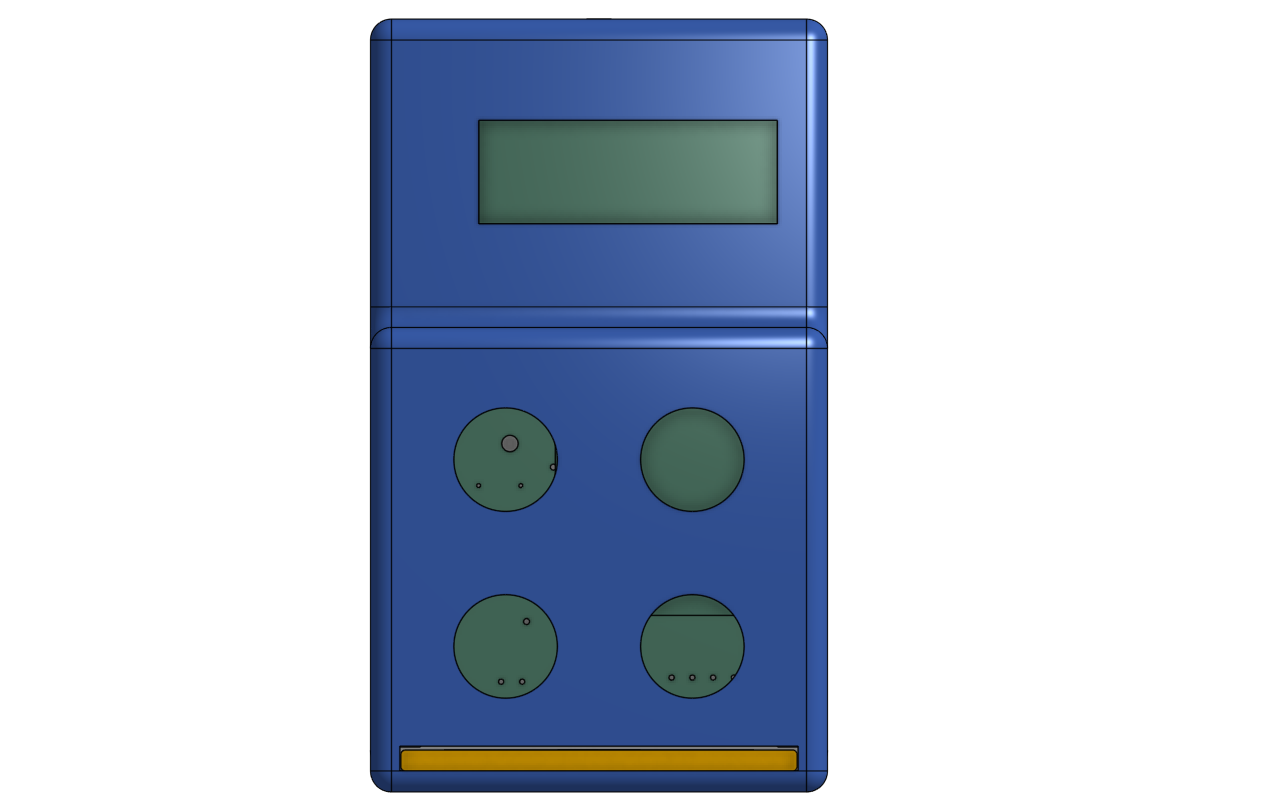
\includegraphics[width=\textwidth]{images/krabickaTop.png}
		\caption{Pohled shora na schránku}
		\label{fig:krabickaTop}
	\end{subfigure}%
	\hfill
	\begin{subfigure}[t]{0.48\textwidth}
		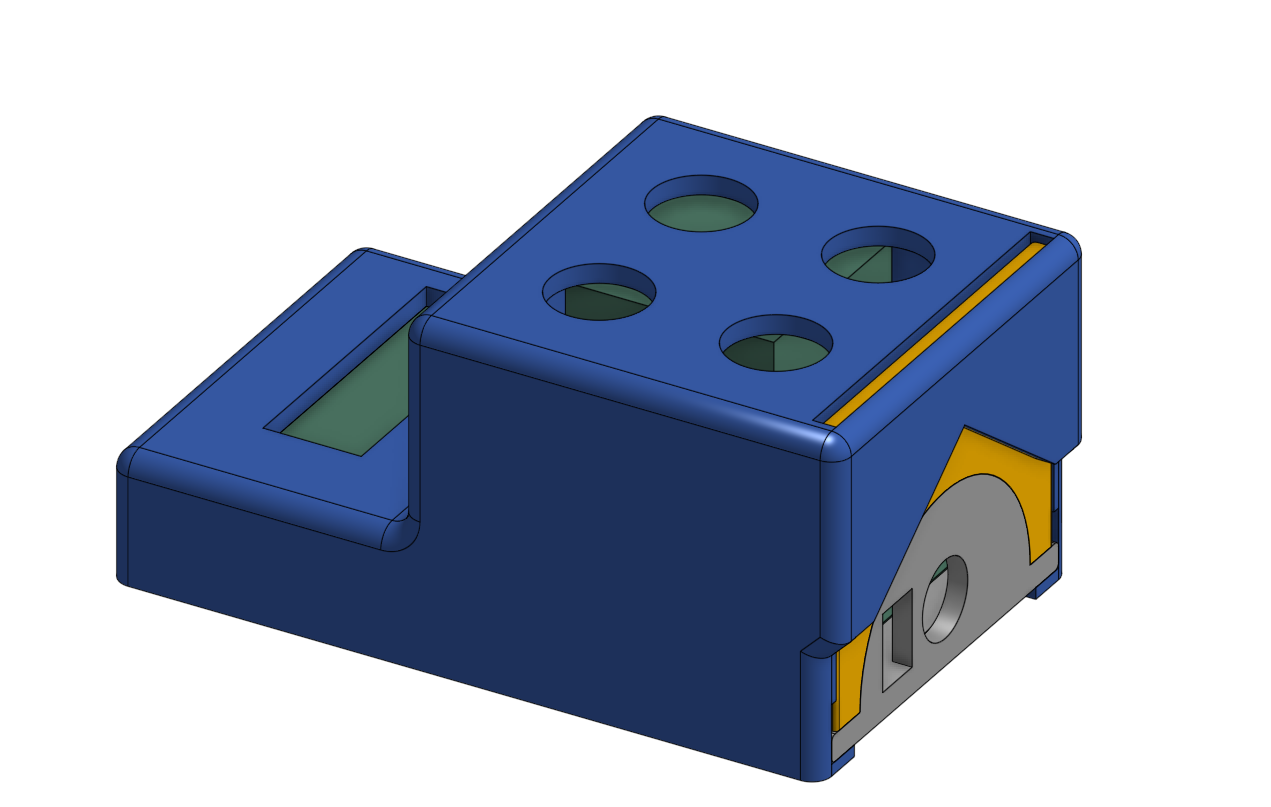
\includegraphics[width=\textwidth]{images/KrabickaZBoku.png}
		\caption{Pohled z boku na schránku}
		\label{fig:KrabickaZBoku}
	\end{subfigure}
	\caption{Model schránky pro desku plošných spojů}
	\label{fig:krabickaObaPohledy}
\end{figure}

Po dokončení modelů v prostředí Onshape byly tiskové soubory exportovány do softwaru Bambu Studio a následně odeslány k tisku na zmíněnou tiskárnu. Pro tisk byl zvolen bílý PETG filament značky SUNLU. Tento materiál byl preferován pro svou vyšší mechanickou odolnost ve srovnání s PLA, přičemž jeho zpracování nevyžaduje náročné tiskové podmínky ani hardware. Během tisku byl tento filament vysoušen kvůli známým problémům s vlhkostí uvnitř PETG filamentu.

\section{Kompletace řešení}
%\purpose{Tady bude postup kompletace celého zařízení a k tomu obrázky, které blíže popisují kde jsou jednotlivé části.}

Během kompletace systému byly nejdříve připájeny veškeré osazované součástky na desku plošných spojů. Následně došlo k připojení dvou komponent, které jsou navržené jako vyjímatelné moduly – vývojová deska WEMOS D1 Mini Pro a LCD displej. Tyto součástky byly navrženy jako snadno vyjímatelné primárně kvůli tomu, že to nejsou standardní zapouzdřené integrované obvody určené přímo k pájení. Jelikož jsou tyto součástky komplexnější, je dobré mít možnost je jednodušeji diagnostikovat a vyměnit, protože můžou vyžadovat složitější nastavení pro optimální funkčnost. Kromě toho je při prototypování vývojová deska často vyjímána kvůli nahrávání firmwaru a ladění kódu během vývoje, zatímco modul LCD displeje disponuje na spodní straně trimrem, který mění kontrast, a ten se typicky také nastavuje až po osazení modulu na desce.

Finální podobu desky plošných spojů lze vidět na obrázku \ref{fig:PCBFinal}.

\begin{figure}[H]
	\centering
	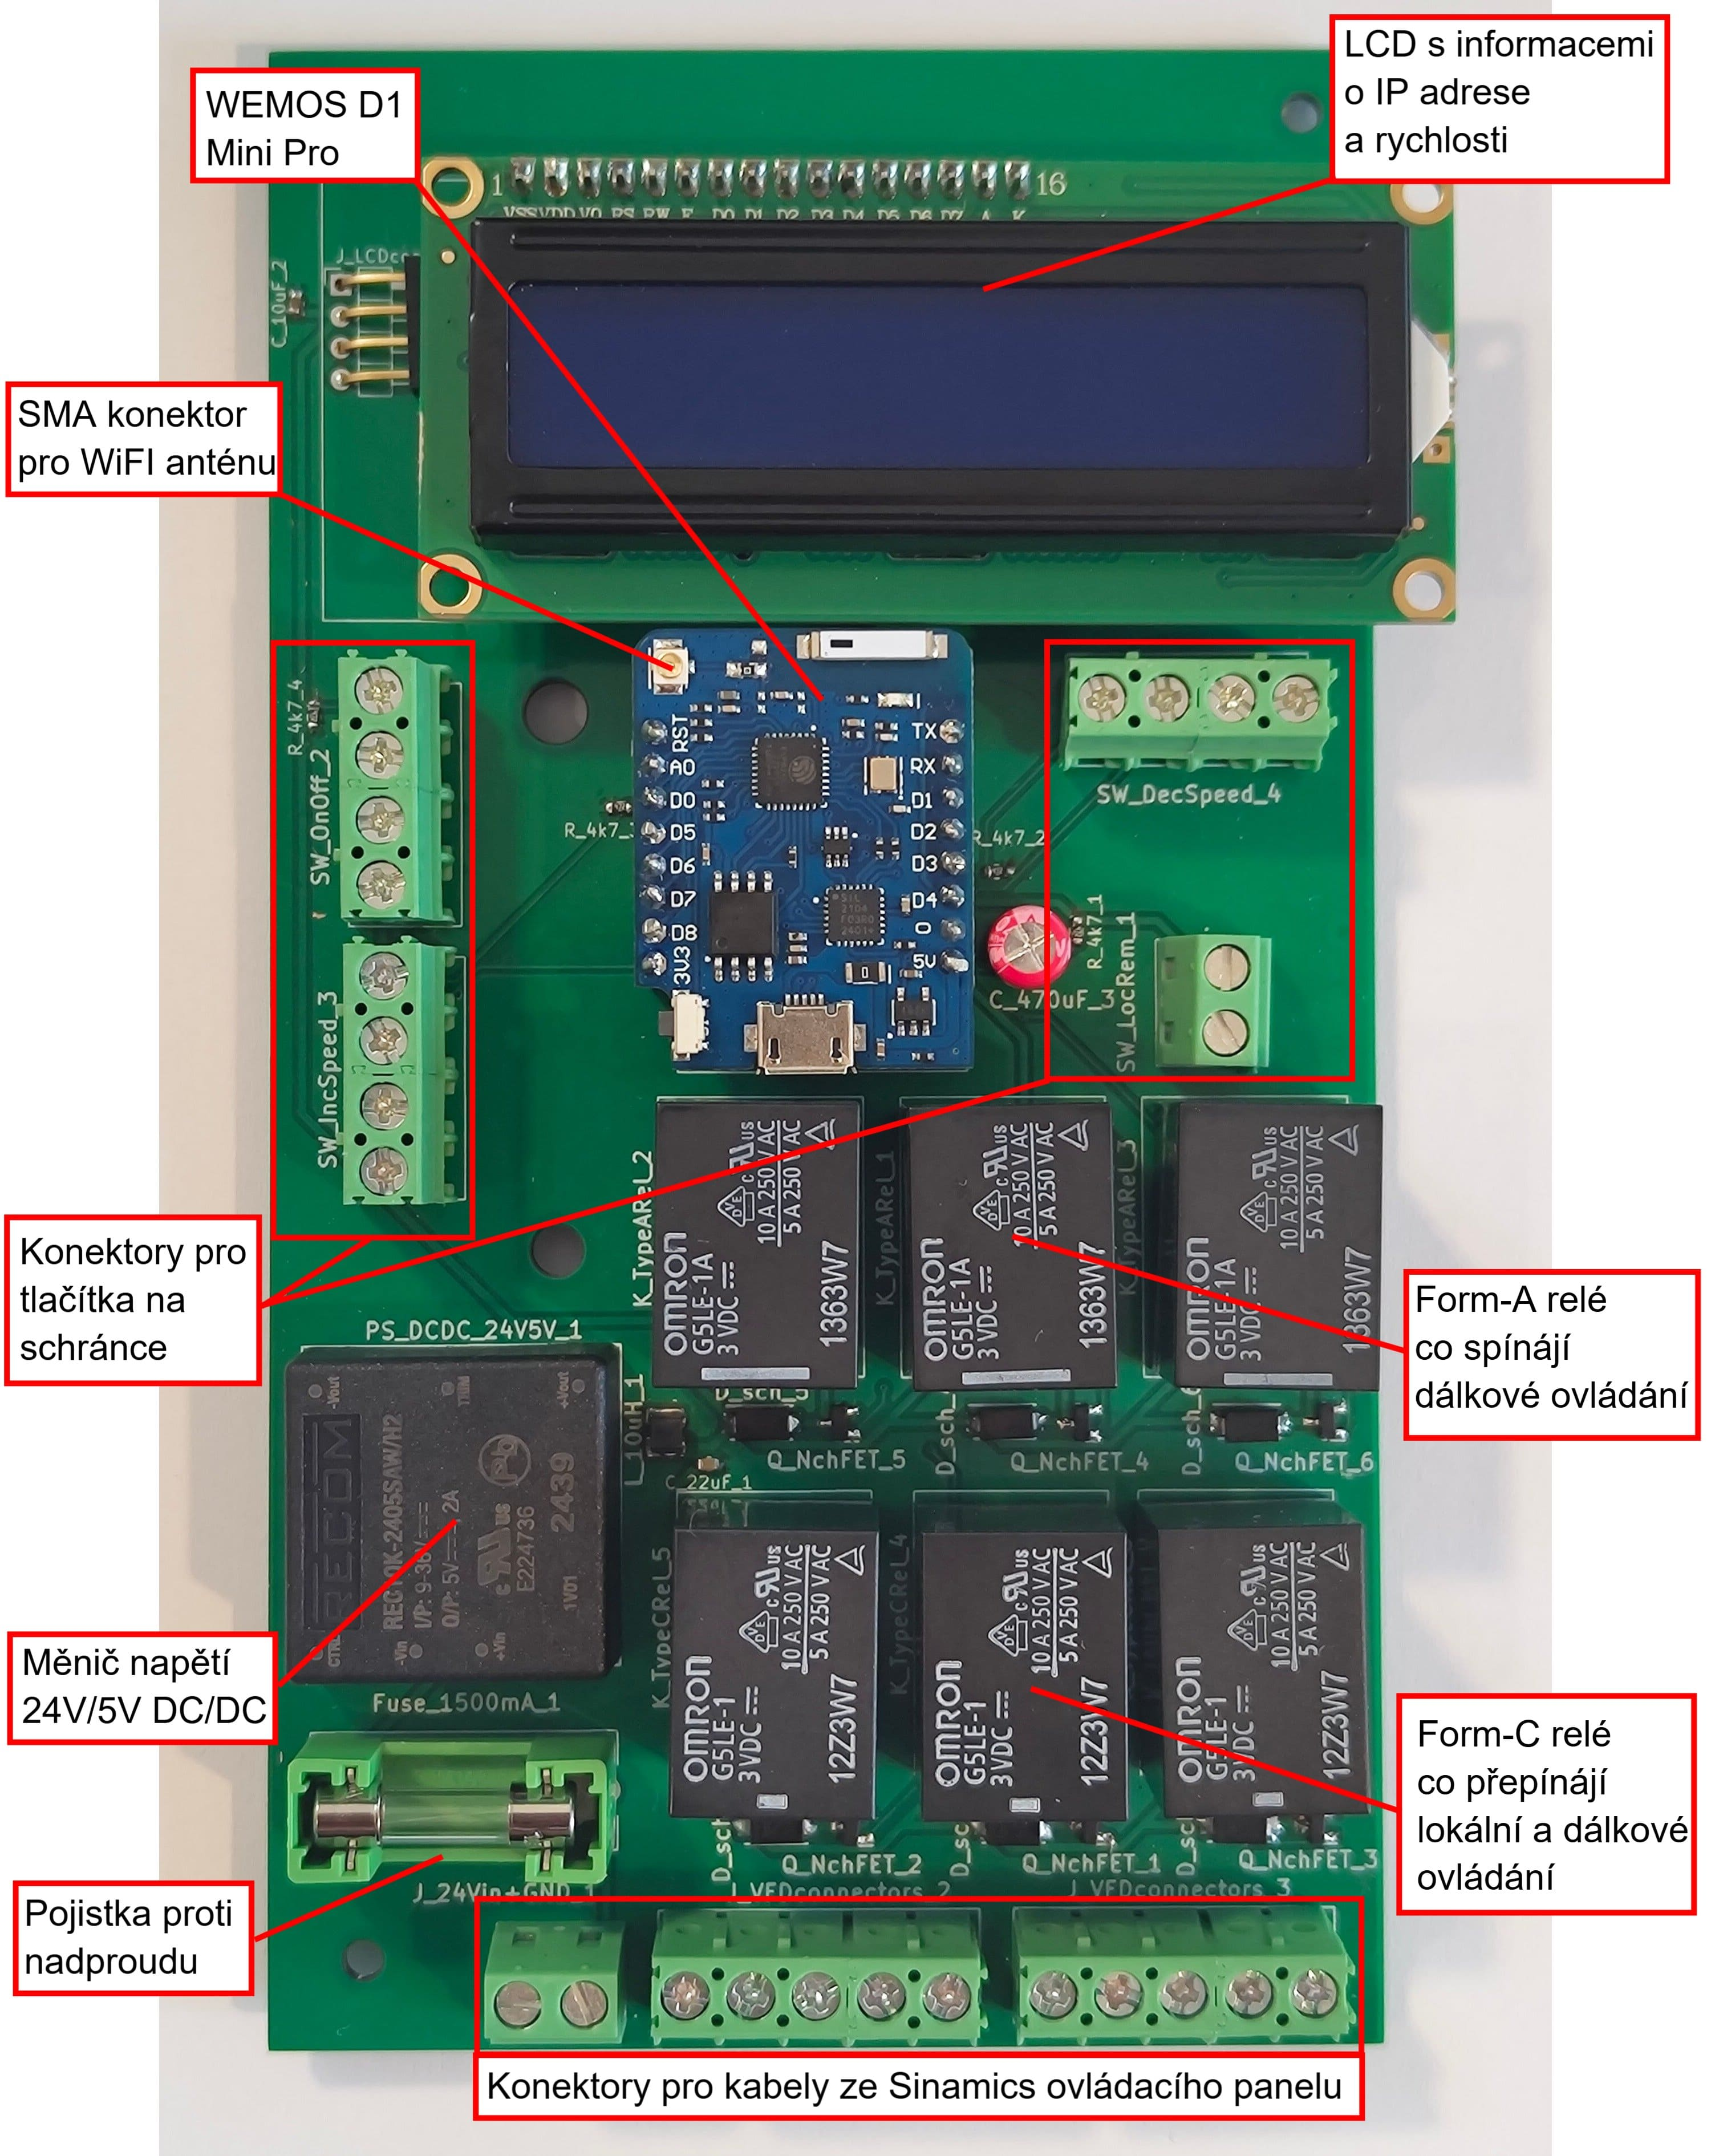
\includegraphics[width=0.95\linewidth]{images/PCB_Final_annotated.jpg}
	\caption{Finální podoba desky plošných spojů}
	\label{fig:PCBFinal}
\end{figure}

Po osazení komponent na DPS je dalším krokem připojení kabelů, které komunikují s ovládacím panelem frekvenčního měniče a napájí vývojovou desku. Tyto kabely se připojují do šroubovacích svorkovnic na spodní straně desky plošných spojů. Následně byla tlačítka umístěna na schránku pro desku a k těmto tlačítkům byly připojeny kabely do šroubovacích konektorů, které jsou umístěné uprostřed desky. Poté je možné upevnit desku ve schránce.

V této fázi je deska připravená pro připojení k dopravníkovému systému, jehož princip je zobrazen na začátku návrhové kapitoly na obrázku \ref{fig:PrincipFunkceZarizeni}. Napájení desky je možné realizovat buď z ovládacího panelu frekvenčního měniče, což je doporučený způsob napájení kvůli jednoduchosti, vzhledem k tomu, že jsou veškeré ostatní kabely také připojené k frekvenčnímu měniči. Systém ale bude fungovat i v případě, že nebude napájen z frekvenčního měniče – desku je možné napojit na libovolný externí zdroj poskytující stejnosměrné napětí v rozsahu $9–48V$. Špičková hodnota proudu, kterou je možné v extrémním případě na DPS zaznamenat, je asi $1,3A$ při $5V$ napájení, takže na vstupu musí zdroj poskytovat při napětí $24V$ kolem $300mA$ proudu.